\documentclass[aspectratio=43,10pt]{beamer}

% =============================================================================
% PPD-II THIRD REVIEW PRESENTATION
% Title: AI-Powered Security Operations Center (SOC) Assistant Using Large Language Models
% Student: Kunal Sanga (2301341031) | Soumili Ghosh (231341057) | Bivan Jena (2301341021)
% Supervisor: Miss Alka Dash, Assistant Professor, Department of CSE
% Institution: Silicon Institute of Technology, Sambalpur
% Template: Custom Silicon Institute of Technology Beamer Design (SKP-beamer compatible)
% Compile with: pdfLaTeX in Overleaf or local TeX distribution
% =============================================================================

\usepackage[utf8]{inputenc}
\usepackage[T1]{fontenc}
\usepackage{lmodern}
\usepackage{graphicx}
\usepackage{xcolor}
\usepackage{tikz}
\usetikzlibrary{calc,positioning,arrows.meta,shadows,fit,shapes.geometric}
\usepackage{booktabs}
\usepackage{colortbl}
\usepackage{tabularx}
\usepackage{array}
\usepackage{ragged2e}
\usepackage{tcolorbox}
\tcbuselibrary{skins}
\usepackage{amsmath,amssymb}

% --- Color Palette Aligned with Template Visual Identity ---
\definecolor{SOCteal}{RGB}{17,94,119}          % Deep academic teal
\definecolor{SOCtealLight}{RGB}{53,145,160}    % Cyan accent
\definecolor{SOCnav}{RGB}{64,64,64}            % Dark gray footer strip
\definecolor{SOCdark}{RGB}{19,51,72}           % Midnight dark text
\definecolor{SOCpale}{RGB}{237,243,247}        % Soft card background
\definecolor{SOCline}{RGB}{207,219,225}        % Card border
\definecolor{SOCgray}{RGB}{93,108,118}         % Muted gray
\definecolor{SOCwhite}{RGB}{255,255,255}
\definecolor{SOCgreen}{RGB}{34,139,74}         % Passing / Verified
\definecolor{SOCamber}{RGB}{210,105,30}        % Pending / Warning
\definecolor{SOCred}{RGB}{185,28,28}           % Error / Contrast
\definecolor{SOCbadgeBg}{RGB}{254,243,199}     % Warning badge background

\usetheme{default}
\setbeamersize{text margin left=0.04\paperwidth,text margin right=0.04\paperwidth}
\setbeamerfont{normal text}{size=\small}
\setbeamercolor{normal text}{fg=SOCdark,bg=white}
\setbeamercolor{structure}{fg=SOCteal}
\setbeamercolor{itemize item}{fg=SOCteal}
\setbeamercolor{itemize subitem}{fg=SOCtealLight}
\setbeamertemplate{navigation symbols}{}
\setbeamertemplate{itemize item}{\raisebox{0.15ex}{\tiny$\blacktriangleright$}}
\setbeamertemplate{itemize subitem}{\raisebox{0.15ex}{\tiny$\blacktriangleright$}}

% Footer strip with dynamic slide counter
\newcommand{\SOCfooter}[1]{%
\begin{tikzpicture}[remember picture,overlay]
  \fill[SOCnav] (current page.south west) rectangle ([yshift=0.28cm]current page.south east);
  \node[anchor=west,text=white,font=\fontsize{5.5}{6.5}\selectfont]
    at ([xshift=0.15cm,yshift=0.14cm]current page.south west)
    {Silicon Institute of Technology, Sambalpur};
  \node[anchor=center,text=white,font=\fontsize{5.5}{6.5}\selectfont]
    at ([yshift=0.14cm]current page.south)
    {AI-Powered SOC Assistant \quad\textbar\quad PPD-II Third Review};
  \node[anchor=east,text=white,font=\fontsize{5.5}{6.5}\selectfont]
    at ([xshift=-0.15cm,yshift=0.14cm]current page.south east)
    {Slide \insertframenumber{} / \inserttotalframenumber};
\end{tikzpicture}%
}

% Clean header bar with institute logo and teal accent
\newcommand{\SOCheading}[2]{%
\begin{tikzpicture}[remember picture,overlay]
  \fill[SOCteal] (current page.north west) rectangle ([yshift=-0.72cm]current page.north east);
  \draw[SOCtealLight,line width=1.5pt] ([yshift=-0.72cm]current page.north west) -- ([yshift=-0.72cm]current page.north east);
  \node[anchor=west,text=white,font=\sffamily\fontsize{11.5}{13.5}\bfseries\selectfont]
    at ([xshift=0.25cm,yshift=-0.26cm]current page.north west) {#1};
  \node[anchor=west,text=SOCpale!95,font=\sffamily\fontsize{7.2}{8.8}\selectfont]
    at ([xshift=0.25cm,yshift=-0.51cm]current page.north west) {#2};
  \node[anchor=east] at ([xshift=-0.25cm,yshift=-0.36cm]current page.north east) {
    \IfFileExists{sitlogo.png}{
\includegraphics[height=0.46cm]{sitlogo.png}}{}
  };
\end{tikzpicture}%
}

% Standard slide wrapper with top alignment and safe vertical clearance below header
\newcommand{\SOCslide}[3]{%
\begin{frame}[t,plain]
\SOCheading{#1}{#2}%
\vspace*{0.68cm}\par
#3
\SOCfooter{\insertframenumber}
\end{frame}
}

% Card component with top colored accent rule and readable padding
\newcommand{\SOCcard}[3]{%
\begin{tikzpicture}
\node[
  draw=SOCline,fill=SOCpale,rounded corners=2.5pt,
  line width=0.5pt,top color=SOCpale,bottom color=white,
  text width={\dimexpr#1-14pt\relax},inner sep=4.5pt,align=left,
  drop shadow={opacity=.05,shadow xshift=0.7pt,shadow yshift=-0.7pt}
] (card) {\textbf{\color{SOCdark}\normalsize#2}\\[2pt]\small #3};
\draw[SOCteal,line width=1.8pt] (card.north west)--(card.north east);
\end{tikzpicture}%
}

% Highlight banner box
\newcommand{\SOCbox}[4]{%
\begin{tikzpicture}
\node[
  draw=#2,fill=#3,rounded corners=2pt,
  line width=0.5pt,text width={\dimexpr#1-14pt\relax},inner sep=3.5pt,align=left
] (box) {\color{SOCdark}#4};
\end{tikzpicture}%
}

\begin{document}

% =============================================================================
% SLIDE 1: Title Page
% =============================================================================
\begin{frame}[plain]
\begin{tikzpicture}[remember picture,overlay]
  \fill[white] (current page.south west) rectangle (current page.north east);
  
  % Teal top banner
  \fill[SOCteal] ([xshift=0.03\paperwidth]current page.north west)
    rectangle ([xshift=-0.03\paperwidth,yshift=-2.00cm]current page.north east);
  \draw[SOCtealLight,line width=2.2pt]
    ([xshift=0.03\paperwidth,yshift=-2.00cm]current page.north west) -- 
    ([xshift=-0.03\paperwidth,yshift=-2.00cm]current page.north east);

  \node[text=white,align=center,text width=.90\paperwidth,font=\sffamily\bfseries\fontsize{13.5}{16.5}\selectfont]
    at ([yshift=-1.00cm]current page.north)
    {AI-Powered Security Operations Center\\(SOC) Assistant Using Large Language Models};

  % Presentation Subtitle & Review Tag
  \node[anchor=north,align=center,font=\sffamily] at ([yshift=-2.22cm]current page.north) {
    {\color{SOCteal}\bfseries\small PPD-II --- THIRD REVIEW PRESENTATION}\\[1.5pt]
    {\color{SOCgray}\scriptsize Milestone Evaluation: Implementation, Benchmark Results, Analysis \& Contributions}
  };

  % Team Members Block
  \node[anchor=north,align=center,font=\sffamily] at ([yshift=-2.98cm]current page.north) {
    {\color{SOCgray}\fontsize{7.5}{9}\selectfont\bfseries PROJECT TEAM}\\[3pt]
    {\textbf{\color{SOCdark}\normalsize Kunal Sanga} \quad {\color{SOCgray}\footnotesize(2301341031)}}\\[1.5pt]
    {\textbf{\color{SOCdark}\normalsize Soumili Ghosh} \quad {\color{SOCgray}\footnotesize(231341057)}}\\[1.5pt]
    {\textbf{\color{SOCdark}\normalsize Bivan Jena} \quad {\color{SOCgray}\footnotesize(2301341021)}}
  };

  % Supervisor Block
  \node[anchor=north,align=center,font=\sffamily] at ([yshift=-4.78cm]current page.north) {
    {\fontsize{7.5}{9}\selectfont\color{SOCtealLight}\bfseries UNDER THE GUIDANCE OF}\\[2.5pt]
    {\fontsize{12.5}{14.5}\selectfont\bfseries\color{SOCdark} Miss Alka Dash}\\[2pt]
    {\footnotesize\color{SOCdark} Assistant Professor, Department of Computer Science \& Engineering}
  };

  % Institution & Date Footer
  \node[anchor=south west,font=\sffamily\footnotesize,text=SOCgray]
    at ([xshift=0.40cm,yshift=0.45cm]current page.south west) {Silicon Institute of Technology, Sambalpur \quad\textbar\quad November 2026};

  % Institute Logo
  \node[anchor=south east] at ([xshift=-0.45cm,yshift=0.35cm]current page.south east)
    {\IfFileExists{sitlogo.png}{
\includegraphics[width=2.3cm]{sitlogo.png}}{}};
\end{tikzpicture}
\end{frame}

% =============================================================================
% SLIDE 2: Problem Statement & Motivation
% =============================================================================
\SOCslide{Problem Statement \& Motivation}{Addressing Critical Alert Fatigue, Triaging Bottlenecks, and Data Privacy in SOCs}{
\begin{columns}[T,onlytextwidth]
\column{0.48\textwidth}
\SOCcard{\linewidth}{The Triage Crisis in Modern SOCs}{
\begin{itemize}\setlength{\itemsep}{2pt}\footnotesize
  \item \textbf{Alert Inundation}: Tier-1 analysts face 1,000+ alerts daily per shift; over 40\% are ignored or superficially closed due to cognitive fatigue.
  \item \textbf{Manual Correlation}: Cross-referencing raw telemetry with MITRE ATT\&CK techniques and NVD CVE catalogs is slow and error-prone.
  \item \textbf{Prolonged Dwell Time}: Severe investigation backlogs delay threat containment, enabling lateral adversary movement.
\end{itemize}
}

\column{0.48\textwidth}
\SOCcard{\linewidth}{Risks of Naive Cloud AI Solutions}{
\begin{itemize}\setlength{\itemsep}{2pt}\footnotesize
  \item \textbf{Data Privacy \& Compliance}: Transmitting internal hostnames, IPs, and user identities to cloud LLMs violates compliance (SOC2/GDPR).
  \item \textbf{Hallucination Risk}: Commercial general-purpose LLMs hallucinate non-existent CVEs and invalid MITRE tactics.
  \item \textbf{Opaque Triage}: Without verifiable citations, analysts cannot trace AI recommendations back to authoritative security documentation.
\end{itemize}
}
\end{columns}

\vspace{0.08cm}
\SOCbox{\linewidth}{SOCline}{SOCpale}{
  \footnotesize\textbf{Research Opportunity:} Build a \textbf{fully sovereign, on-premise AI assistant} that couples entity-anchored retrieval with local open-weights LLMs to produce citation-grounded, audit-ready security triage without cloud data egress.
}
}

% =============================================================================
% SLIDE 3: Project Objectives
% =============================================================================
\SOCslide{Project Objectives}{Clear Engineering and Research Goals for the AI-Powered SOC Assistant}{
\begin{columns}[T,onlytextwidth]
\column{0.48\textwidth}
\SOCcard{\linewidth}{Core Functional Objectives}{
\begin{itemize}\setlength{\itemsep}{2.5pt}\footnotesize
  \item \textbf{Autonomous Advisory Triage}: Deliver plain-English incident summaries, threat severity ratings, and prioritized containment actions in real time.
  \item \textbf{Evidence-Grounded Reasoning}: Ground all LLM assertions directly in authoritative knowledge (MITRE ATT\&CK Enterprise Matrix + NVD CVE repository).
  \item \textbf{Audit-Ready Citation Verification}: Enforce automated validation of every cited evidence ID to eliminate fabricated references before persistence.
\end{itemize}
}

\column{0.48\textwidth}
\SOCcard{\linewidth}{Architectural \& System Scope}{
\begin{itemize}\setlength{\itemsep}{2.5pt}\footnotesize
  \item \textbf{Sovereign On-Premise Execution}: Deploy local LLMs (Ollama \texttt{qwen3:8b}) and local vector search (Qdrant) with zero external network dependencies.
  \item \textbf{Interactive Investigation Console}: React 19 UI providing real-time Server-Sent Events (SSE) streaming and interactive entity graph exploration.
  \item \textbf{Human-in-the-Loop Authority}: Serve strictly as an advisory copilot; final containment decisions remain with the human security analyst.
\end{itemize}
}
\end{columns}

\vspace{0.08cm}
\SOCbox{\linewidth}{SOCline}{white}{
  \footnotesize\textbf{Guiding Principle:} The system functions as an \textbf{audit-ready copilot} for human analysts, replacing unassisted manual triage with evidence-backed explanations and verifiable citations.
}
}

% =============================================================================
% SLIDE 4: System Architecture & Technology Stack
% =============================================================================
\SOCslide{System Architecture}{Four-Tier Sovereign On-Premise Pipeline: Ingestion to Interactive UI}{
\begin{center}
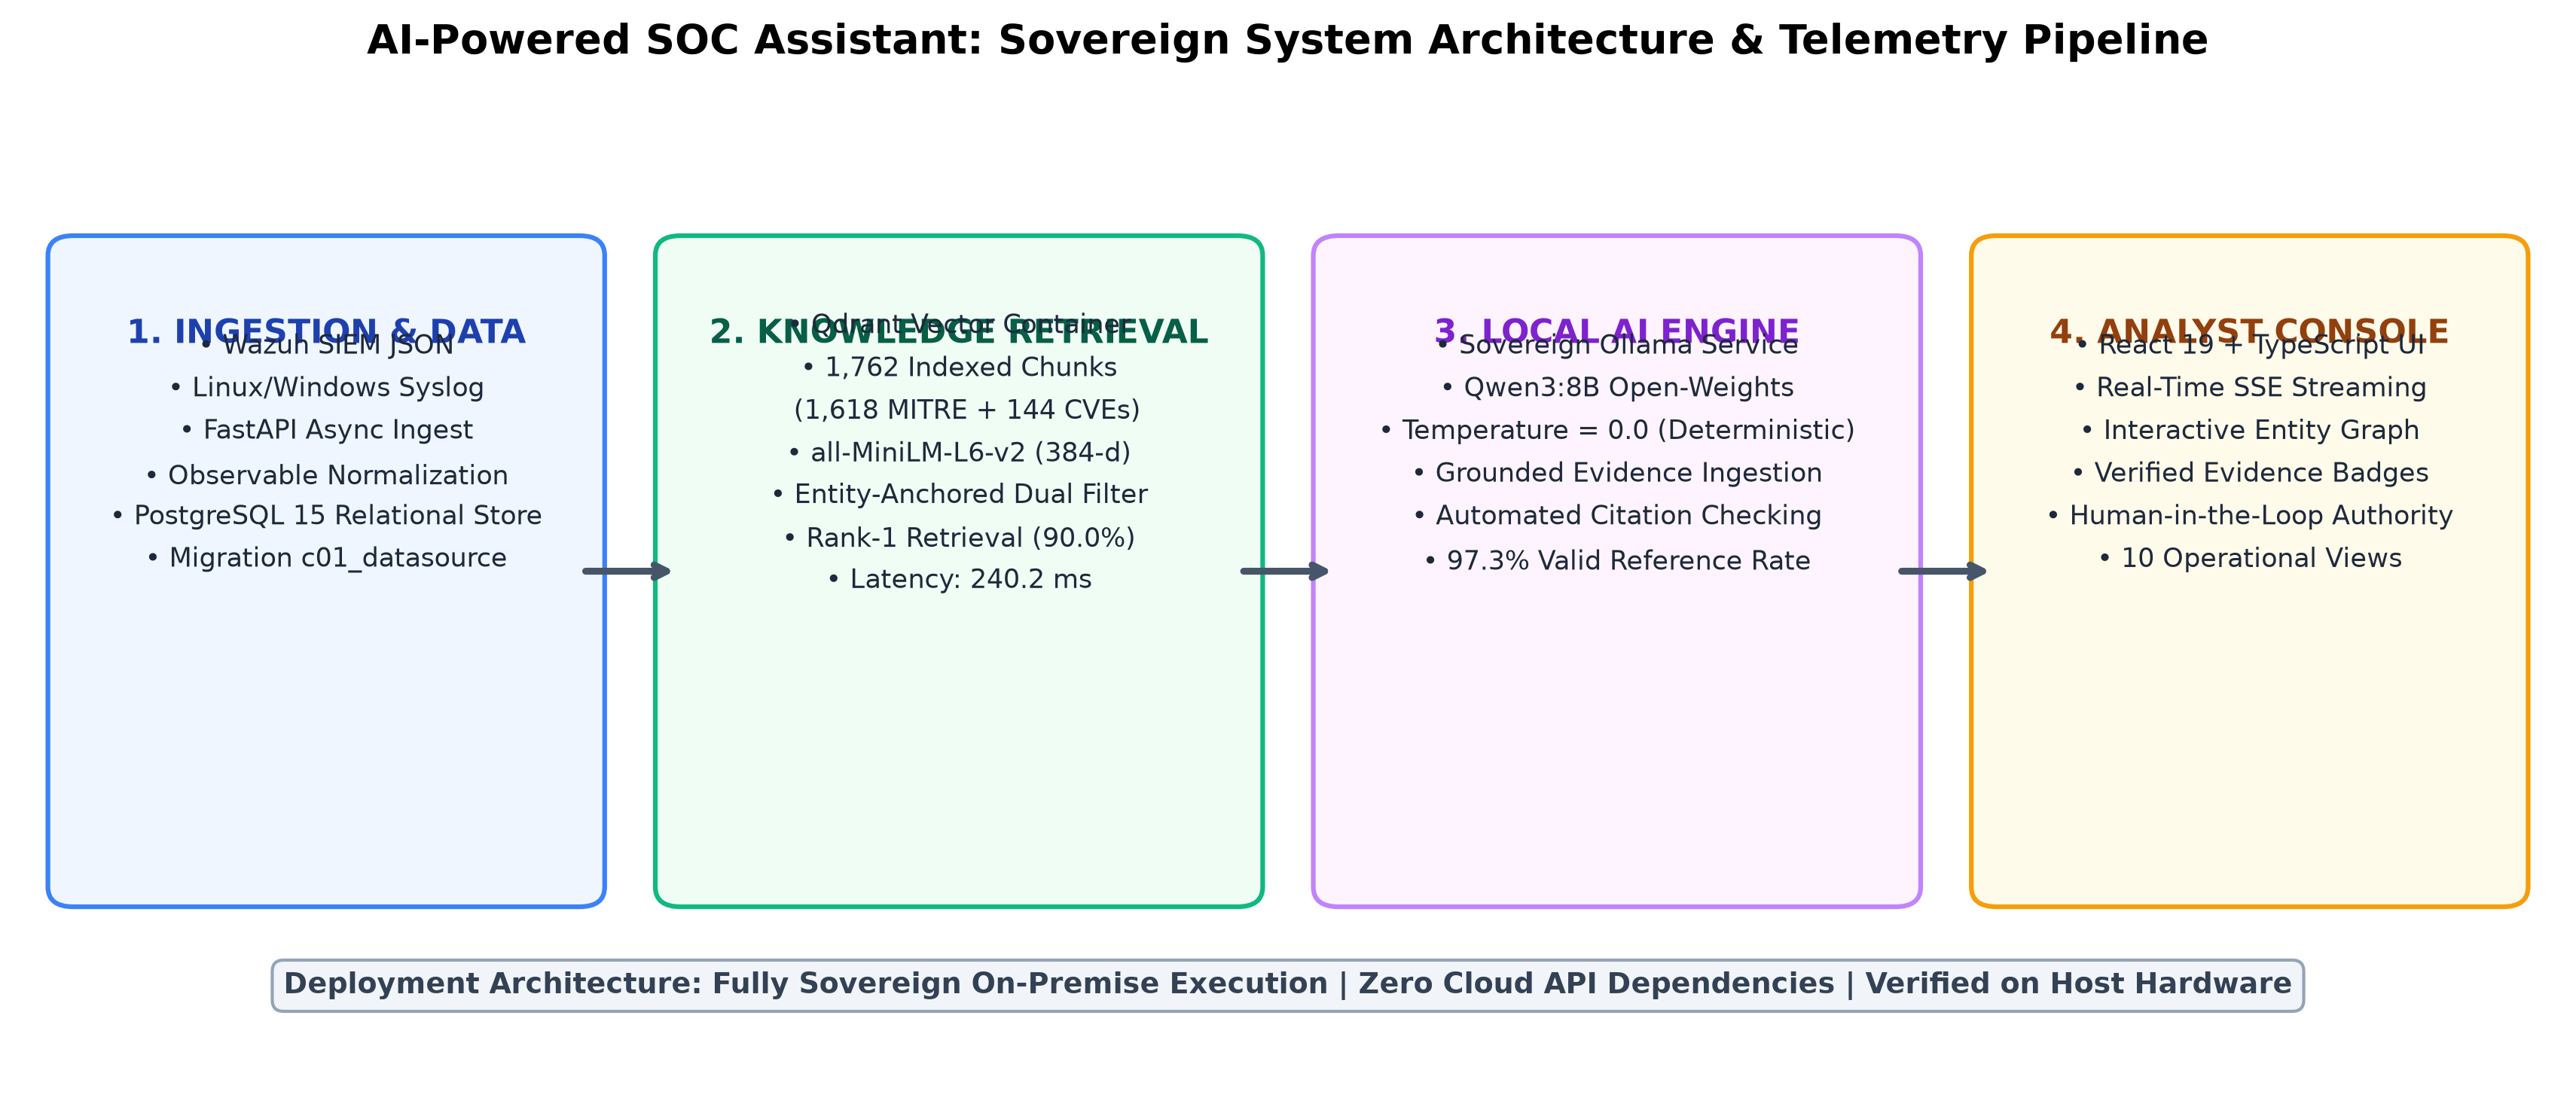
\includegraphics[width=0.98\linewidth,height=5.2cm,keepaspectratio]{figures/architecture_diagram.png}
\end{center}

\vspace{-0.15cm}
\SOCbox{\linewidth}{SOCline}{SOCpale}{
  \footnotesize\textbf{Implementation Reality:} Fully sovereign local deployment (Ollama Qwen3:8B, Qdrant, PostgreSQL 15, React 19). SIEM transport client implemented and tested in mock/replay mode; remote live SIEM validation planned for final defense.
}
}

% =============================================================================
% SLIDE 5: Implementation Completion: Third Review Status
% =============================================================================
\SOCslide{Implementation Completion}{Status of Core Subsystems and Engineering Deliverables for Review 3}{
\begin{columns}[T,onlytextwidth]
\column{0.48\textwidth}
\SOCcard{\linewidth}{Backend \& Knowledge Infrastructure}{
\begin{itemize}\setlength{\itemsep}{2pt}\footnotesize
  \item \textbf{FastAPI Asynchronous Core}: 21 operational REST and SSE endpoints; live execution trace streaming.
  \item \textbf{PostgreSQL Store}: Alembic migration \texttt{c01\_datasource} applied; strict data-source separation (Demo, Live, Replay).
  \item \textbf{Qdrant Vector Store}: 1,762 chunks indexed with payload metadata and cosine distance metrics.
  \item \textbf{SIEM Connectors}: OpenSearch/Wazuh transport client implemented and operational in verified mock/replay mode.
\end{itemize}
}

\column{0.48\textwidth}
\SOCcard{\linewidth}{Frontend \& Evaluation Framework}{
\begin{itemize}\setlength{\itemsep}{2pt}\footnotesize
  \item \textbf{React 19 Frontend}: 10 production views (Alert Queue, Triage View, Graph Explorer, Trace Stream, Knowledge Navigator).
  \item \textbf{Automated Benchmark Runner}: Multi-mode evaluation harness with SQLite/JSON persistence and checkpoint recovery.
  \item \textbf{Integrity Safeguards}: Dataset namespacing (\texttt{v2-eval-xxx}) eliminates data collision with historical records.
  \item \textbf{Automated Test Suite}: \textcolor{SOCgreen}{\textbf{258 tests passing}} (226 backend unit/integration, 32 frontend Vitest).
\end{itemize}
}
\end{columns}

\vspace{0.08cm}
\SOCbox{\linewidth}{SOCline}{SOCpale}{
  \footnotesize\textbf{Review 3 Milestone Status:} Complete end-to-end implementation verified. All components operate locally on host hardware without external cloud API dependencies.
}
}

% =============================================================================
% SLIDE 6: Three Analysis Modes
% =============================================================================
\SOCslide{Tri-Mode Analysis Paradigm}{Controlled Comparison Across Three Operational Architectures}{
\begin{columns}[T,onlytextwidth]
\column{0.32\textwidth}
\SOCcard{\linewidth}{1. LLM-Only (Zero-Shot)}{
\begin{itemize}\setlength{\itemsep}{2pt}\scriptsize
  \item Raw alert telemetry passed directly to \texttt{qwen3:8b}.
  \item No external retrieval context provided.
  \item Evaluates raw parametric knowledge and memorization.
  \item Vulnerable to factual hallucination and temporal decay.
\end{itemize}
}

\column{0.32\textwidth}
\SOCcard{\linewidth}{2. Standard RAG (Dense)}{
\begin{itemize}\setlength{\itemsep}{2pt}\scriptsize
  \item Alert text embedded via \texttt{all-MiniLM-L6-v2}.
  \item Top-5 chunks retrieved via unanchored cosine similarity.
  \item Retrieved text prepended to prompt context.
  \item Prone to \textbf{semantic drift} on generic log syntax.
\end{itemize}
}

\column{0.32\textwidth}
\SOCcard{\linewidth}{3. Evidence-Aware RAG}{
\begin{itemize}\setlength{\itemsep}{2pt}\scriptsize
  \item \textbf{Entity extraction} (IPs, users, commands, rule tags).
  \item \textbf{Entity-anchored search} with targeted payload filters.
  \item Injects grounded evidence into prompt template.
  \item \textbf{Citation verification} checks referenced IDs before persistence.
\end{itemize}
}
\end{columns}

\vspace{0.08cm}
\SOCbox{\linewidth}{SOCline}{white}{
  \footnotesize\textbf{Experimental Control:} All three modes are evaluated on identical alert data, using the same local \texttt{qwen3:8b} model, temperature 0.0, and identical system prompt instructions.
}
}

% =============================================================================
% SLIDE 7: Entity-Anchored Retrieval Innovation
% =============================================================================
\SOCslide{Technical Innovation: Entity Anchoring}{Eliminating Semantic Drift in Cybersecurity Log Retrieval}{
\begin{columns}[T,onlytextwidth]
\column{0.48\textwidth}
\SOCcard{\linewidth}{The Flaw in Standard Dense RAG}{
\begin{itemize}\setlength{\itemsep}{2.5pt}\footnotesize
  \item \textbf{Syntactic Dominance}: Security logs are dominated by generic tokens (``failed'', ``connection'', ``user'', ``sshd'', ``port'').
  \item \textbf{Semantic Drift}: Dense embedding vectors match common networking terms rather than adversary techniques.
  \item \textbf{Rank Degradation}: Ground-truth threat techniques are buried deep in candidate lists:
    \begin{itemize}\scriptsize
      \item Standard RAG Recall@1: \textcolor{SOCred}{\textbf{22.5\%}} (9/40).
      \item Standard RAG MRR: \textcolor{SOCred}{\textbf{0.2742}}.
    \end{itemize}
\end{itemize}
}

\column{0.48\textwidth}
\SOCcard{\linewidth}{Our Entity-Anchored Dual Retrieval}{
\begin{itemize}\setlength{\itemsep}{2.5pt}\footnotesize
  \item \textbf{Entity Extraction}: Parses observable entities (IPs, accounts, hashes) and rule metadata tags (\texttt{rule.mitre.id}).
  \item \textbf{Hybrid Filter Generation}: Couples semantic similarity with targeted payload metadata filters.
  \item \textbf{Targeted Re-Ranking}: Pinpoints exact threat techniques directly at Rank 1:
    \begin{itemize}\scriptsize
      \item Evidence-Aware Recall@1: \textcolor{SOCgreen}{\textbf{90.0\%}} (36/40).
      \item Evidence-Aware MRR: \textcolor{SOCgreen}{\textbf{0.9125}}.
    \end{itemize}
\end{itemize}
}
\end{columns}

\vspace{0.08cm}
\SOCbox{\linewidth}{SOCline}{SOCpale}{
  \footnotesize\textbf{Key Breakthrough:} Entity anchoring delivers an absolute \textbf{+67.5 percentage-point leap in Recall@1} over standard dense RAG, ensuring the LLM is supplied with authoritative threat documentation.
}
}

% =============================================================================
% SLIDE 8: Dataset v2 Experimental Methodology
% =============================================================================
\SOCslide{Experimental Methodology}{Dataset v2: Curated 40-Scenario Benchmark with Strict Data Isolation}{
\begin{columns}[T,onlytextwidth]
\column{0.48\textwidth}
\SOCcard{\linewidth}{Dataset v2 Scenario Composition}{
\begin{itemize}\setlength{\itemsep}{1.5pt}\footnotesize
  \item \textbf{40 Diverse Scenarios}: Structured enterprise alerts covering 9 ATT\&CK tactical categories and 1 benign control group:
    \begin{itemize}\scriptsize
      \item \textbf{36 Realistic Attacks}: SSH brute force, Log4Shell RCE, process hollowing, systemd persistence, data exfiltration, ransomware impact.
      \item \textbf{4 Benign Controls}: Authorized Nessus vulnerability scan, admin SSH, scheduled backup rsync, PowerShell module update.
    \end{itemize}
  \item \textbf{Ground Truth}: Curated MITRE techniques and CVEs based on operational Wazuh rule metadata.
\end{itemize}
}

\column{0.48\textwidth}
\SOCcard{\linewidth}{Execution Protocol \& Safeguards}{
\begin{itemize}\setlength{\itemsep}{1.5pt}\footnotesize
  \item \textbf{120 Total Evaluations}: 40 scenarios $\times$ 3 modes evaluated to 100\% completion with \textbf{0 runtime errors}.
  \item \textbf{Data Collision Prevention}: Dataset-namespaced IDs (\texttt{v2-eval-001} to \texttt{v2-eval-040}) eliminate collisions with historical v1 data.
  \item \textbf{Strict Ground-Truth Isolation}: Benchmark runner isolates ground truth; no test contamination during LLM generation.
  \item \textbf{Reproducibility}: Deterministic execution on local Ollama \texttt{qwen3:8b} at temperature 0.0 with full trajectory logging.
\end{itemize}
}
\end{columns}

\vspace{0.04cm}
\SOCbox{\linewidth}{SOCline}{white}{
  \footnotesize\textbf{Integrity Audit:} Evaluated run \texttt{20261109-185423-0f4cfd} independently audited. All raw logs, JSON predictions, and CSV tables are preserved in repository version control.
}
}

% =============================================================================
% SLIDE 9: MITRE ATT&CK Classification Results
% =============================================================================
\SOCslide{MITRE ATT\&CK Classification Results}{End-to-End Technique Classification Across 36 Attack Scenarios}{
\begin{center}
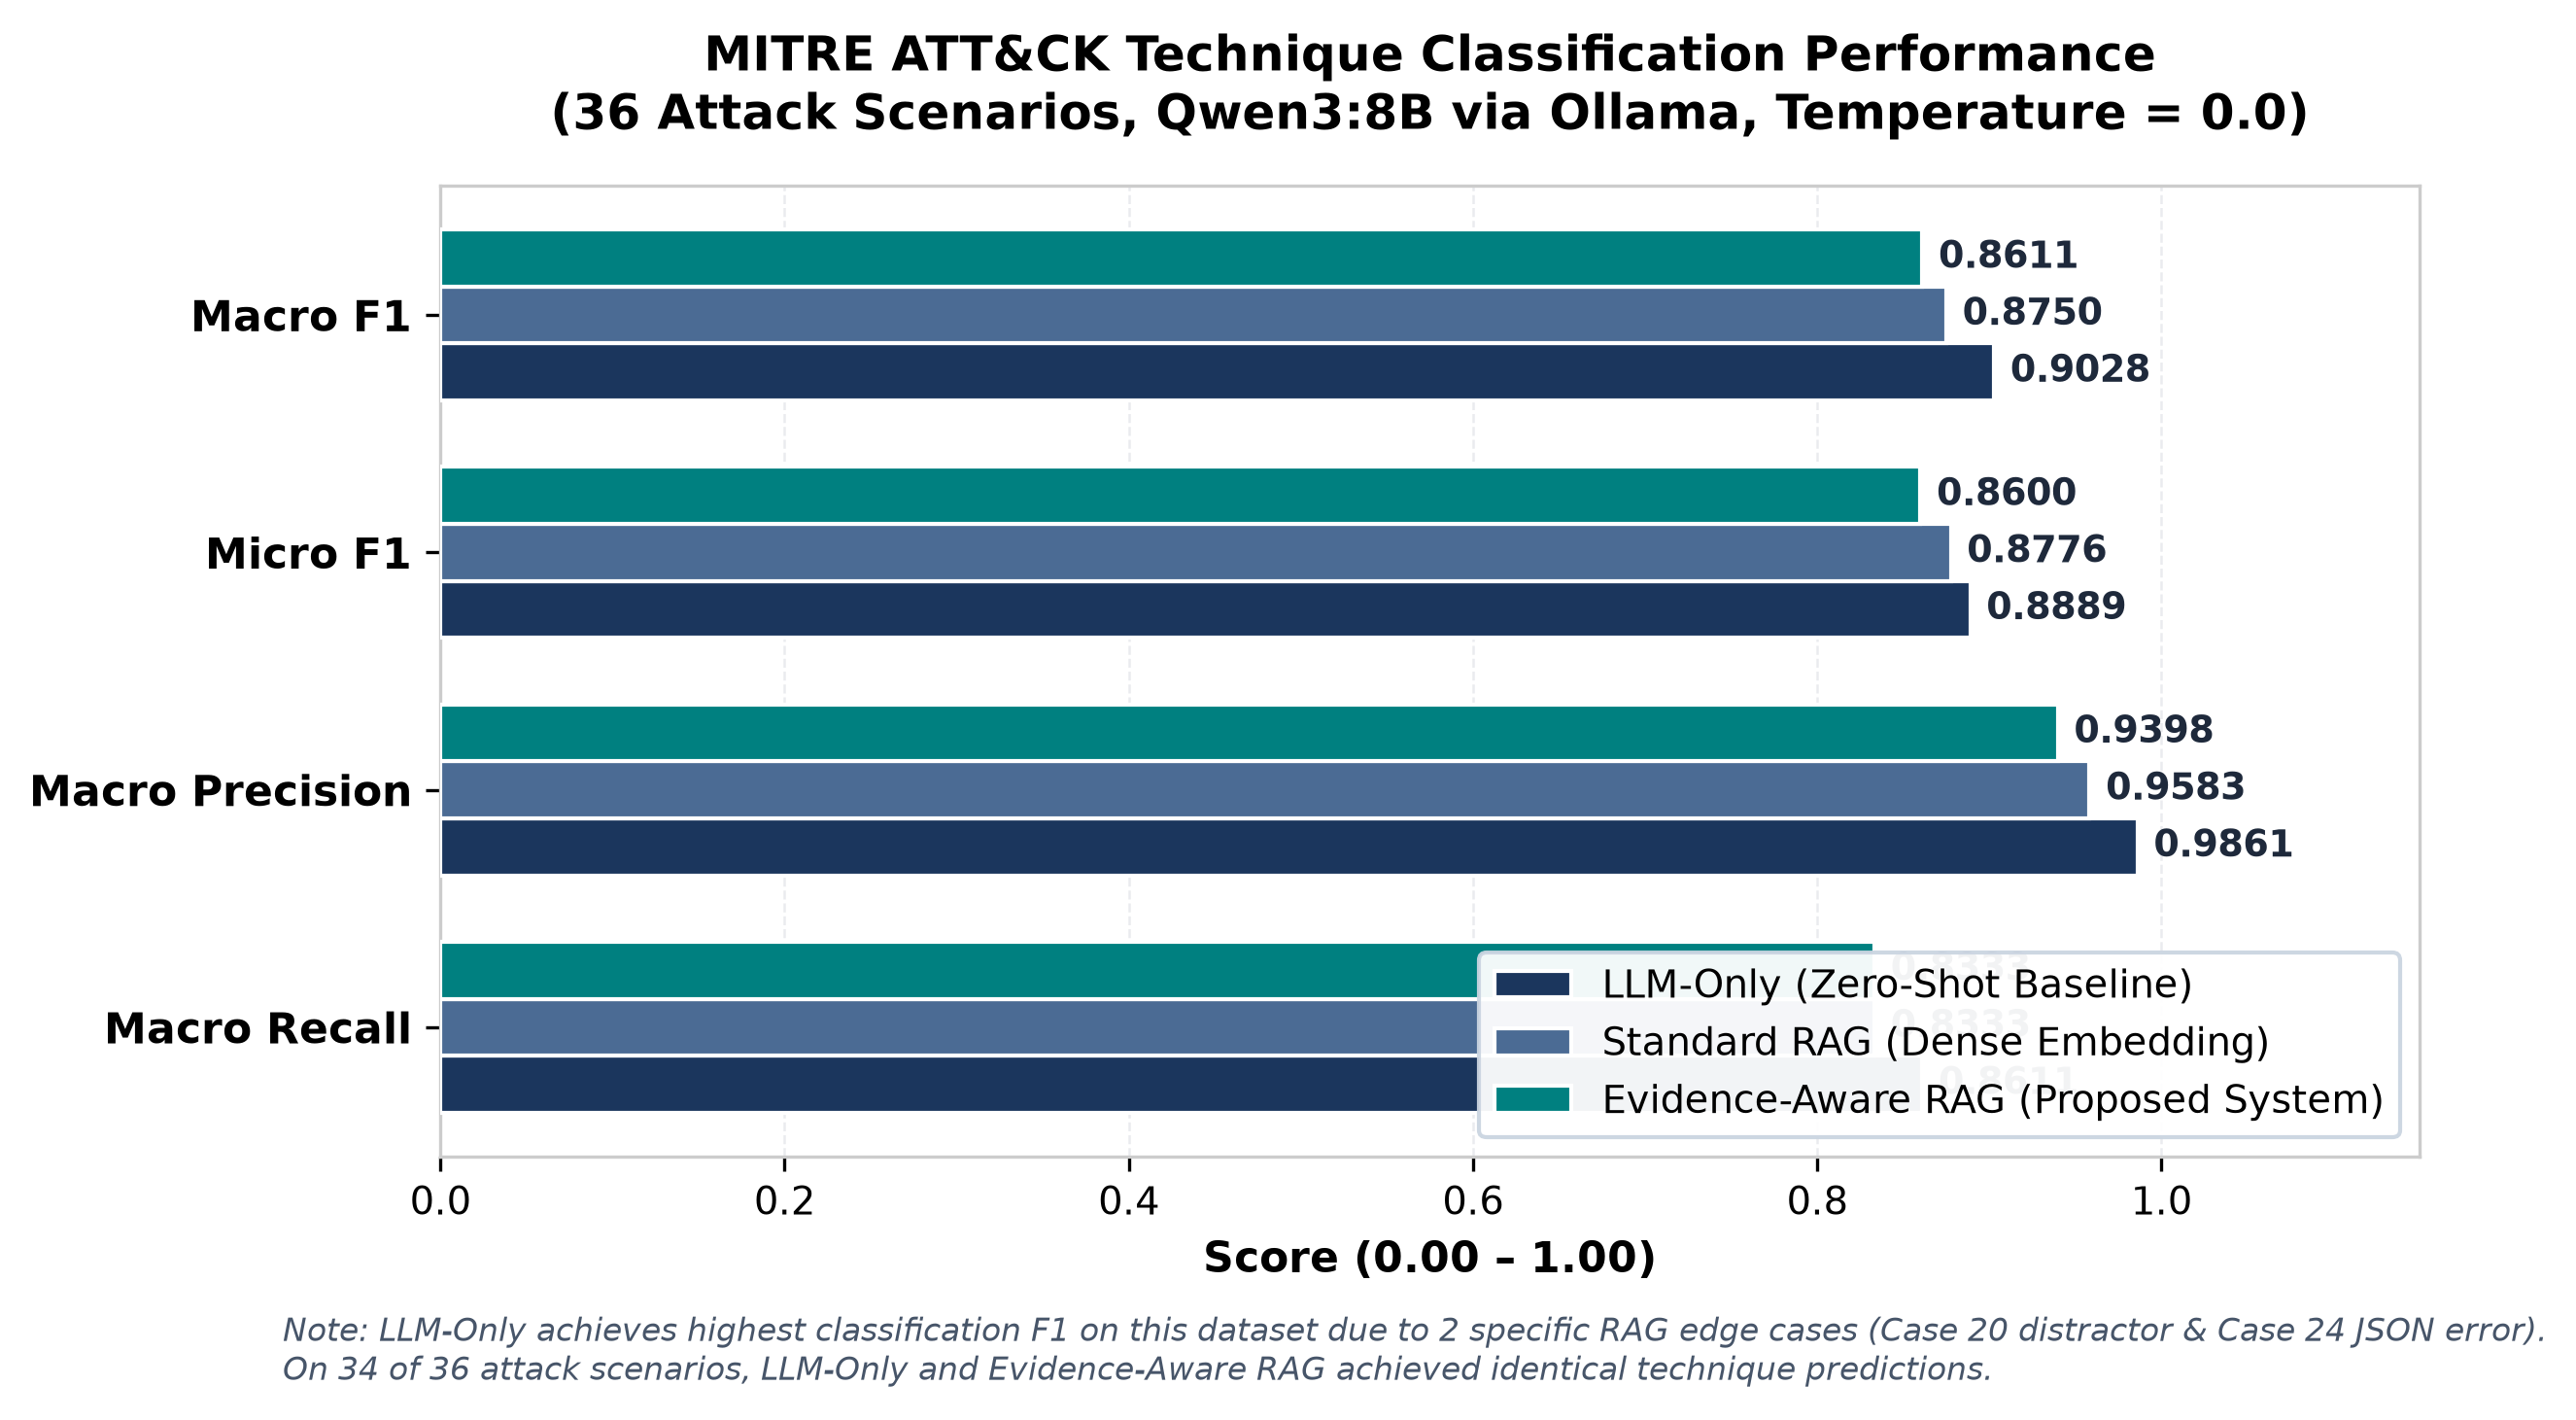
\includegraphics[width=0.96\linewidth,height=4.6cm,keepaspectratio]{figures/figure1_classification.png}
\end{center}

\vspace{-0.15cm}
\SOCbox{\linewidth}{SOCline}{SOCpale}{
  \scriptsize\textbf{Scientific Reality:} Zero-shot LLM achieves highest classification F1 ($0.9028$ vs $0.8611$). On 34 of 36 attack scenarios, predictions were identical; the entire performance gap is caused by Case 20 (context distractor, 2 FPs) and Case 24 (JSON error, 0 predictions). Evidence-Aware's value is verified grounding and retrieval accuracy, not higher classification F1.
}
}

% =============================================================================
% SLIDE 10: Retrieval Ablation Results
% =============================================================================
\SOCslide{Retrieval Ablation Results}{40-Scenario Isolated Retrieval Ablation Over 1,762 Security Chunks (No LLM)}{
\begin{center}
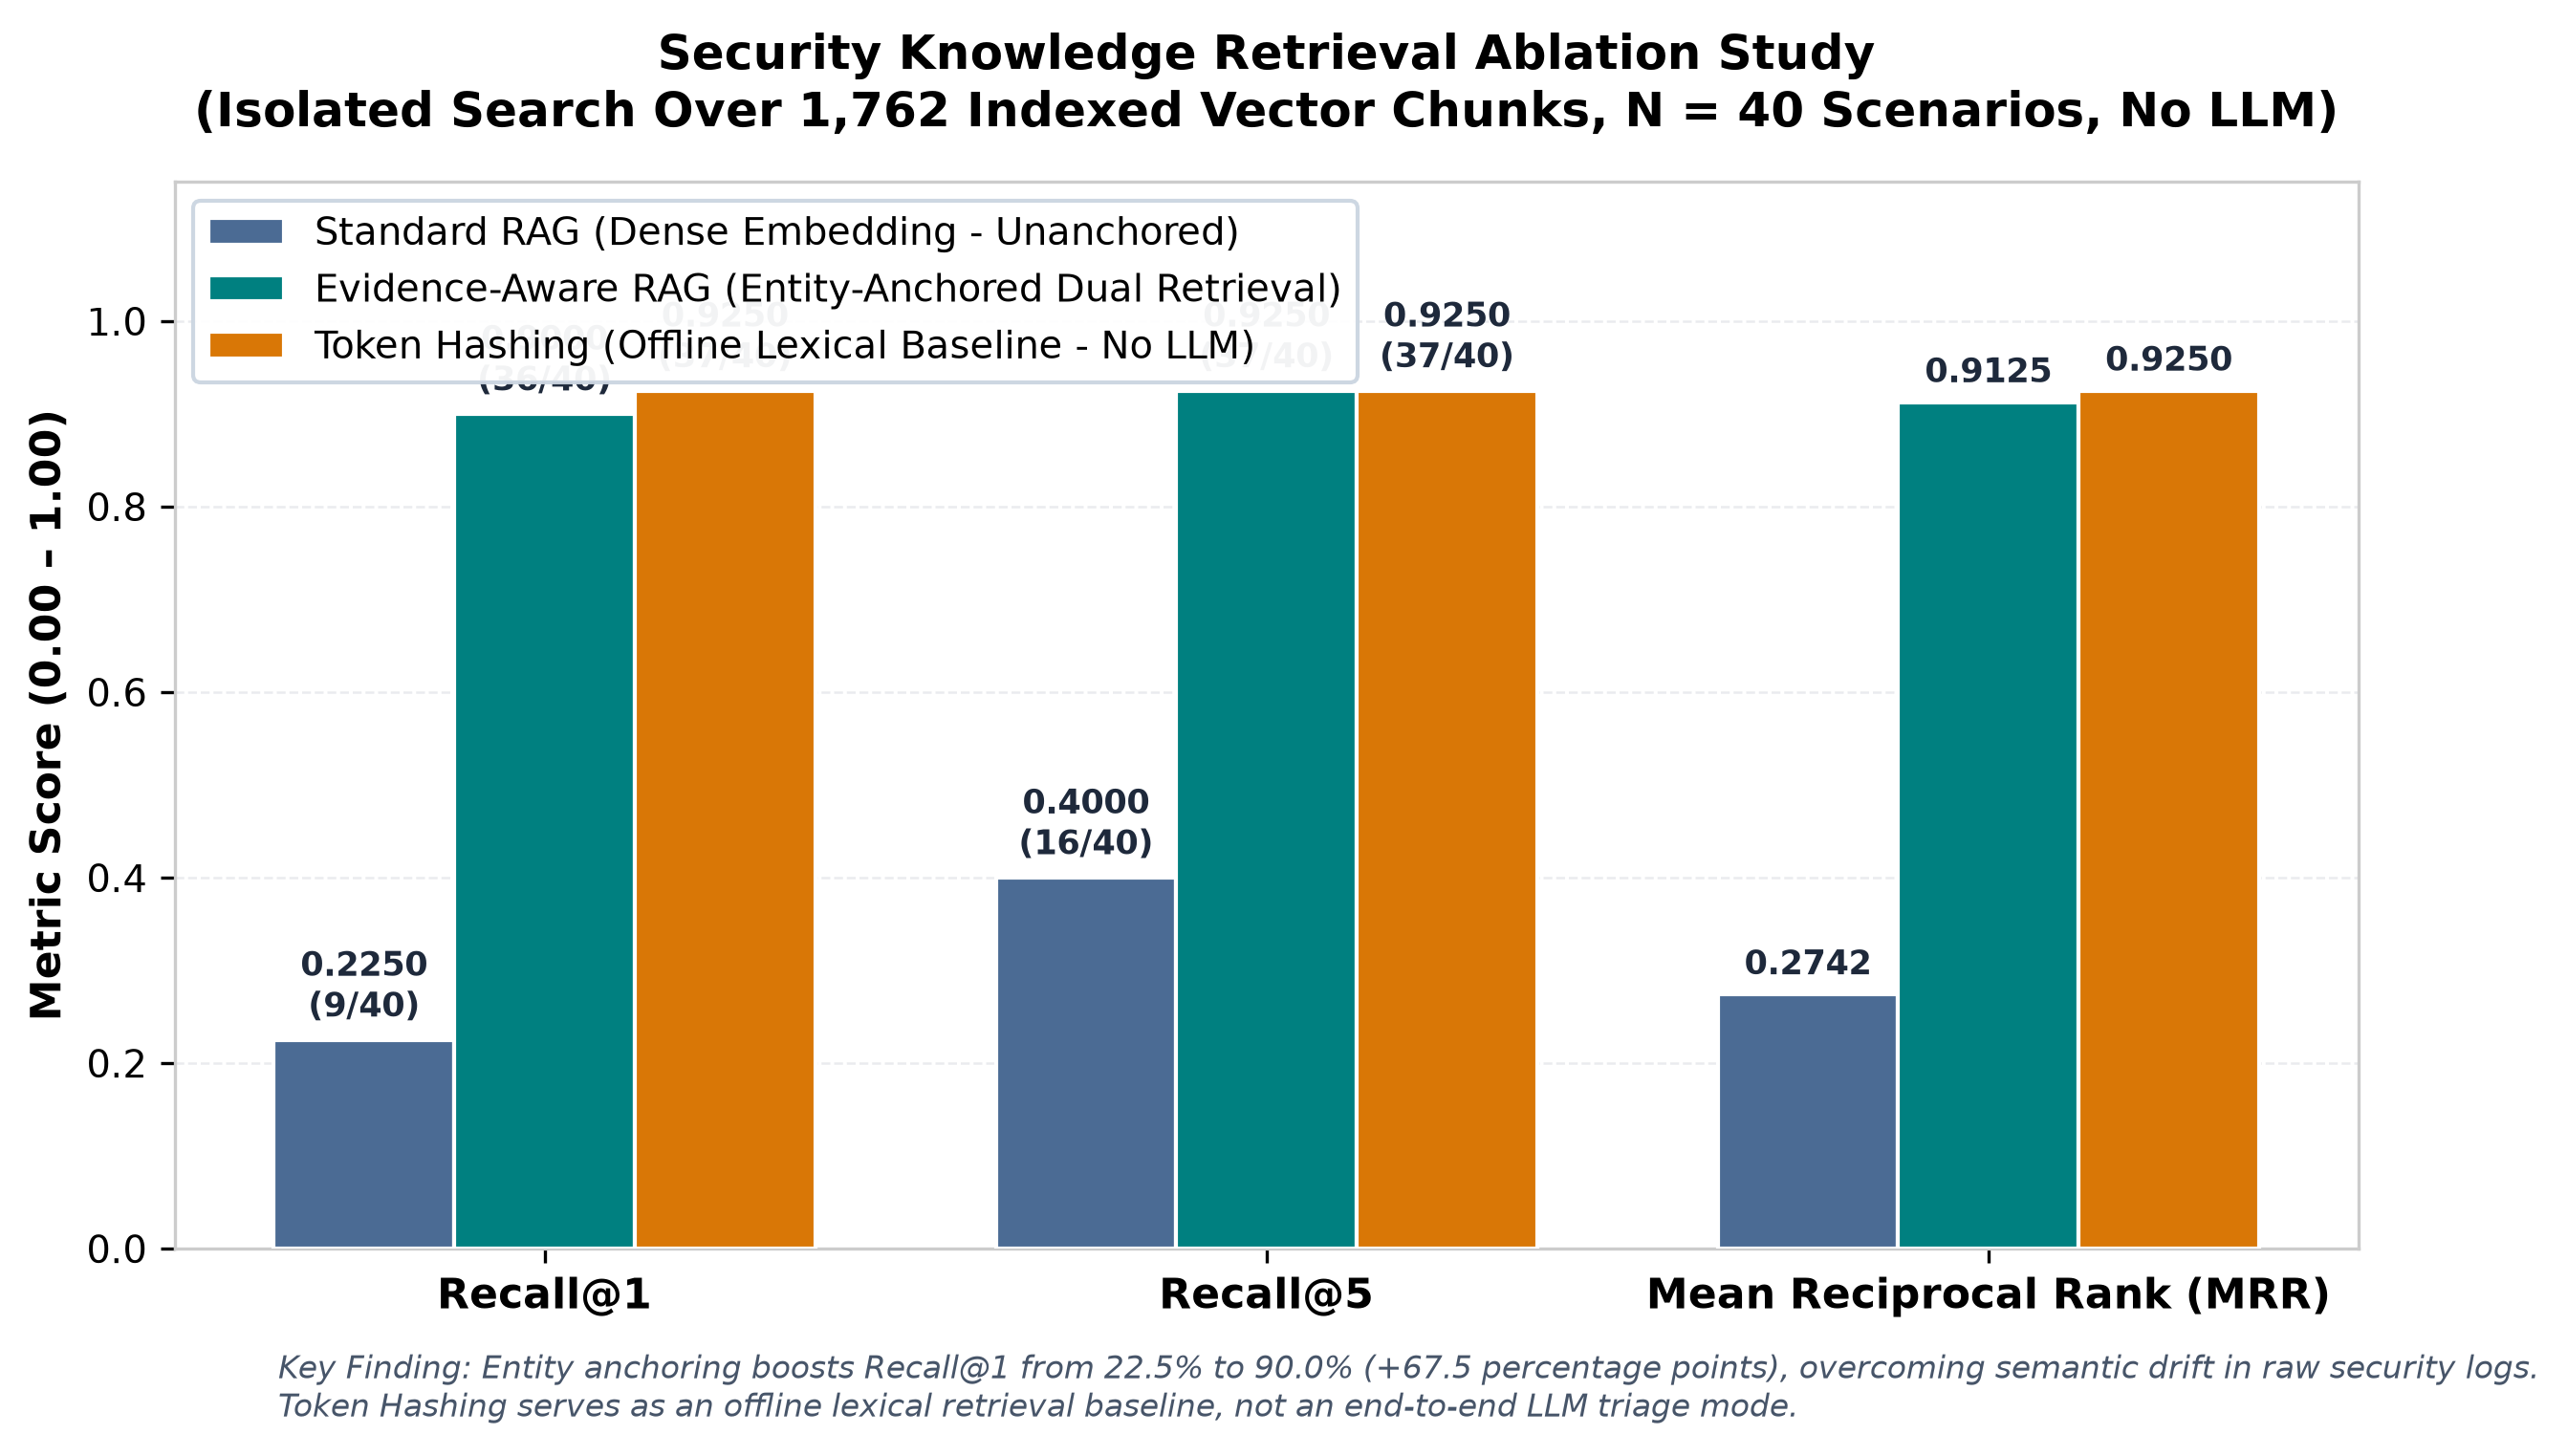
\includegraphics[width=0.96\linewidth,height=4.6cm,keepaspectratio]{figures/figure2_retrieval_ablation.png}
\end{center}

\vspace{-0.15cm}
\SOCbox{\linewidth}{SOCline}{SOCpale}{
  \scriptsize\textbf{Ablation Breakthrough:} Entity anchoring solves semantic drift in security logs, boosting Recall@1 by \textbf{+67.5 percentage points} ($90.0\%$ vs $22.5\%$) and MRR from $0.2742$ to $0.9125$. Token Hashing ($92.5\%$) serves as an offline lexical retrieval baseline (no LLM), not as an end-to-end analysis mode.
}
}

% =============================================================================
% SLIDE 11: Latency Comparison
% =============================================================================
\SOCslide{Latency Comparison: Search vs. Generation}{Clear Separation of Millisecond Knowledge Search from Multi-Second LLM Triage}{
\begin{columns}[T,onlytextwidth]
\column{0.48\textwidth}
\begin{center}
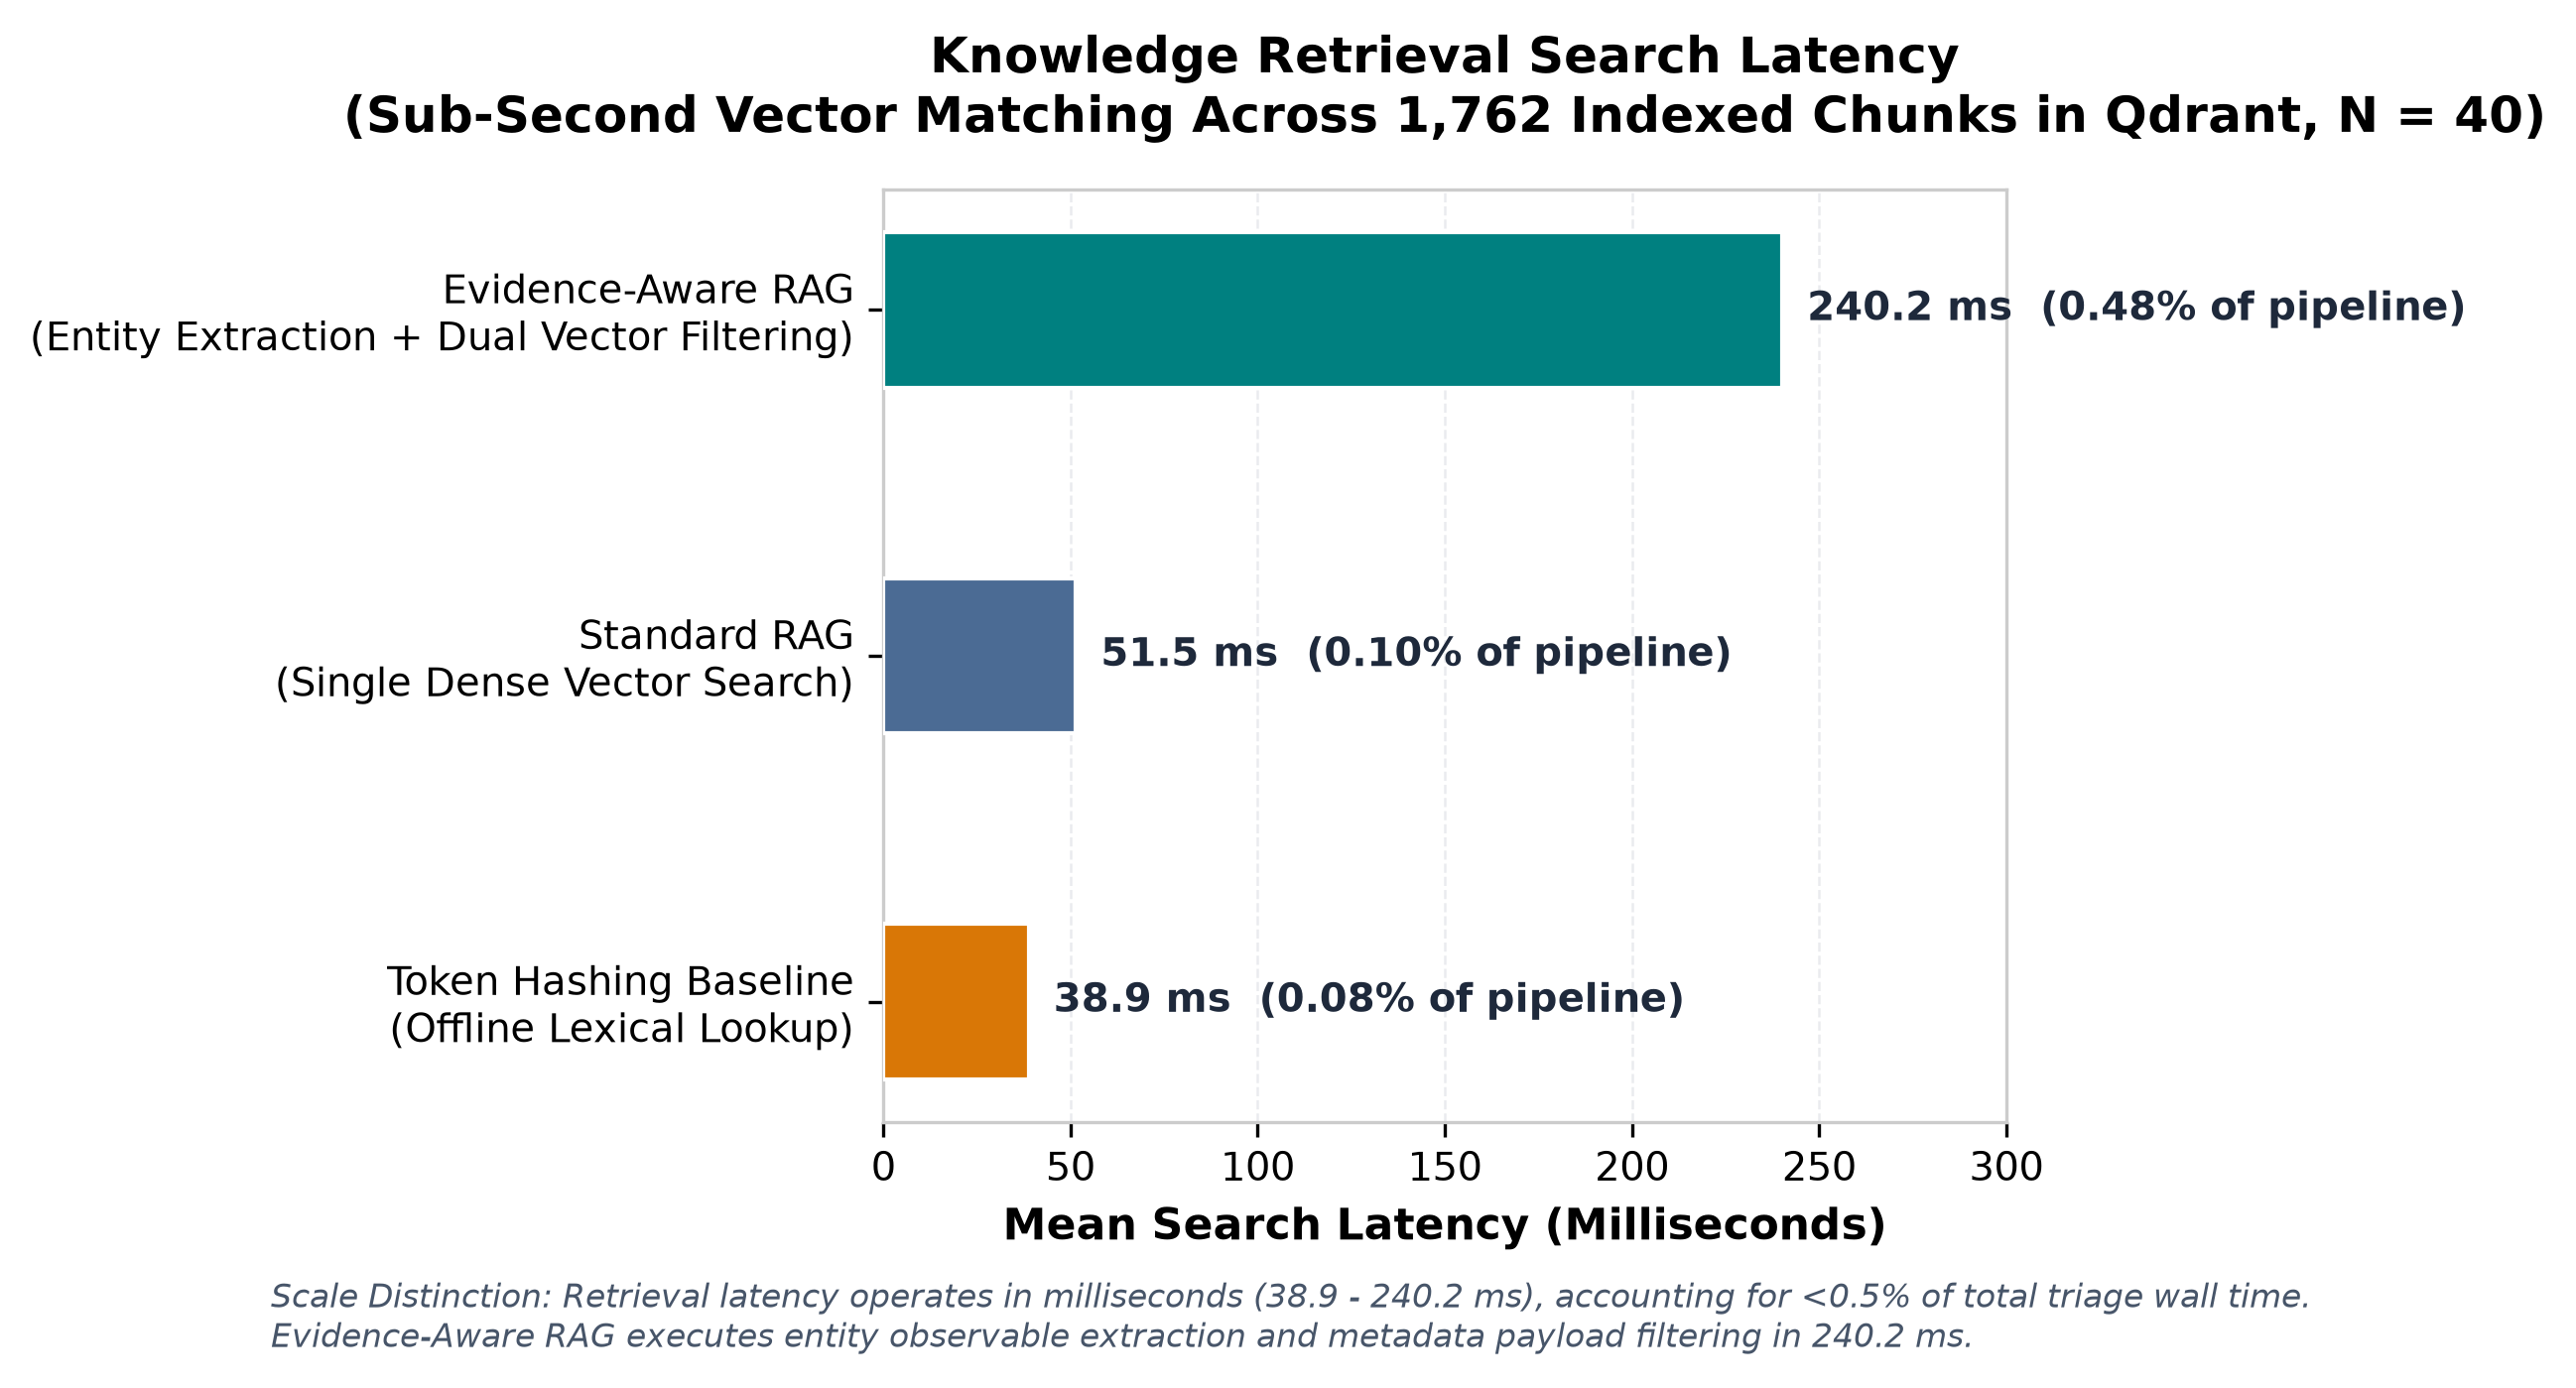
\includegraphics[width=\linewidth,height=4.6cm,keepaspectratio]{figures/figure4_retrieval_latency.png}
\end{center}

\column{0.48\textwidth}
\begin{center}
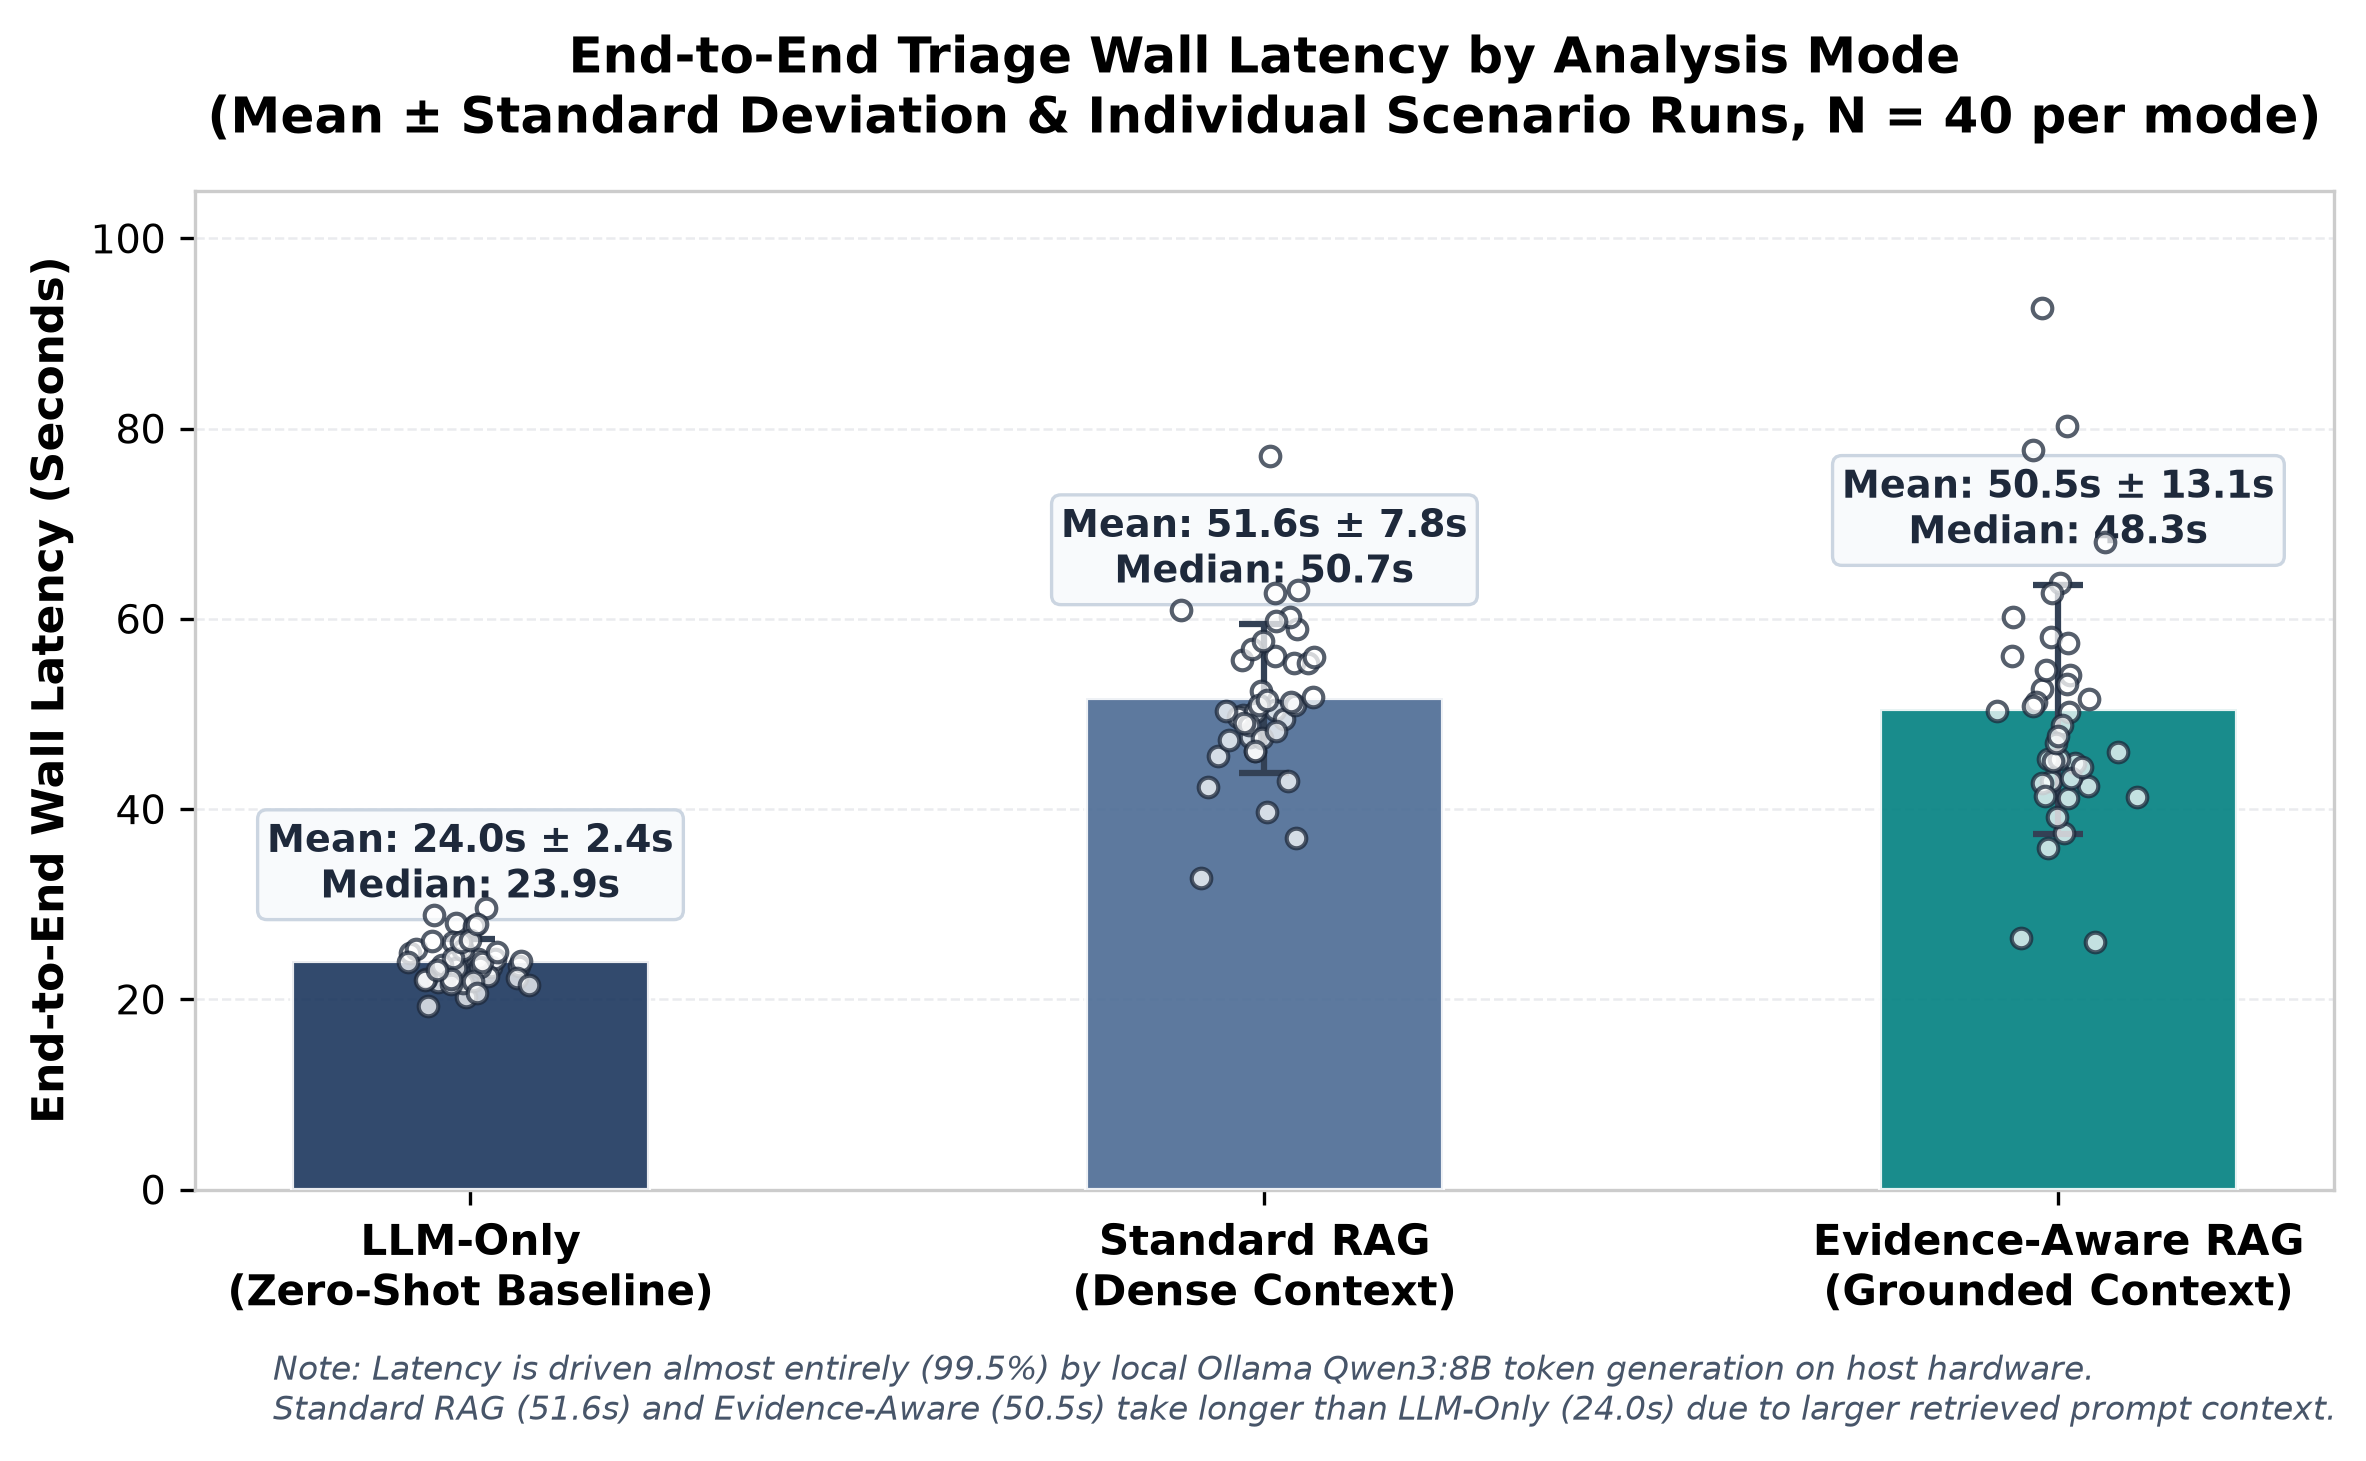
\includegraphics[width=\linewidth,height=4.6cm,keepaspectratio]{figures/figure3_end_to_end_latency.png}
\end{center}
\end{columns}

\vspace{-0.15cm}
\SOCbox{\linewidth}{SOCline}{SOCpale}{
  \scriptsize\textbf{Two Distinct Timing Regimes:} Knowledge retrieval runs in milliseconds ($38.9\text{--}240.2\text{ ms}$, $<0.5\%$ of wall time), whereas local Ollama 8B LLM generation accounts for $99.5\%$ of latency ($24\text{--}51\text{ s}$), completely viable for asynchronous Tier-1 triage queues.
}
}

% =============================================================================
% SLIDE 12: Scenario Category Performance Heatmap
% =============================================================================
\SOCslide{Scenario-Level Performance Heatmap}{Individual Scenario Evaluation ($N = 40$ Cases $\times$ 3 Modes = 120 Evaluations)}{
\begin{columns}[T,onlytextwidth]
\column{0.44\textwidth}
\begin{center}
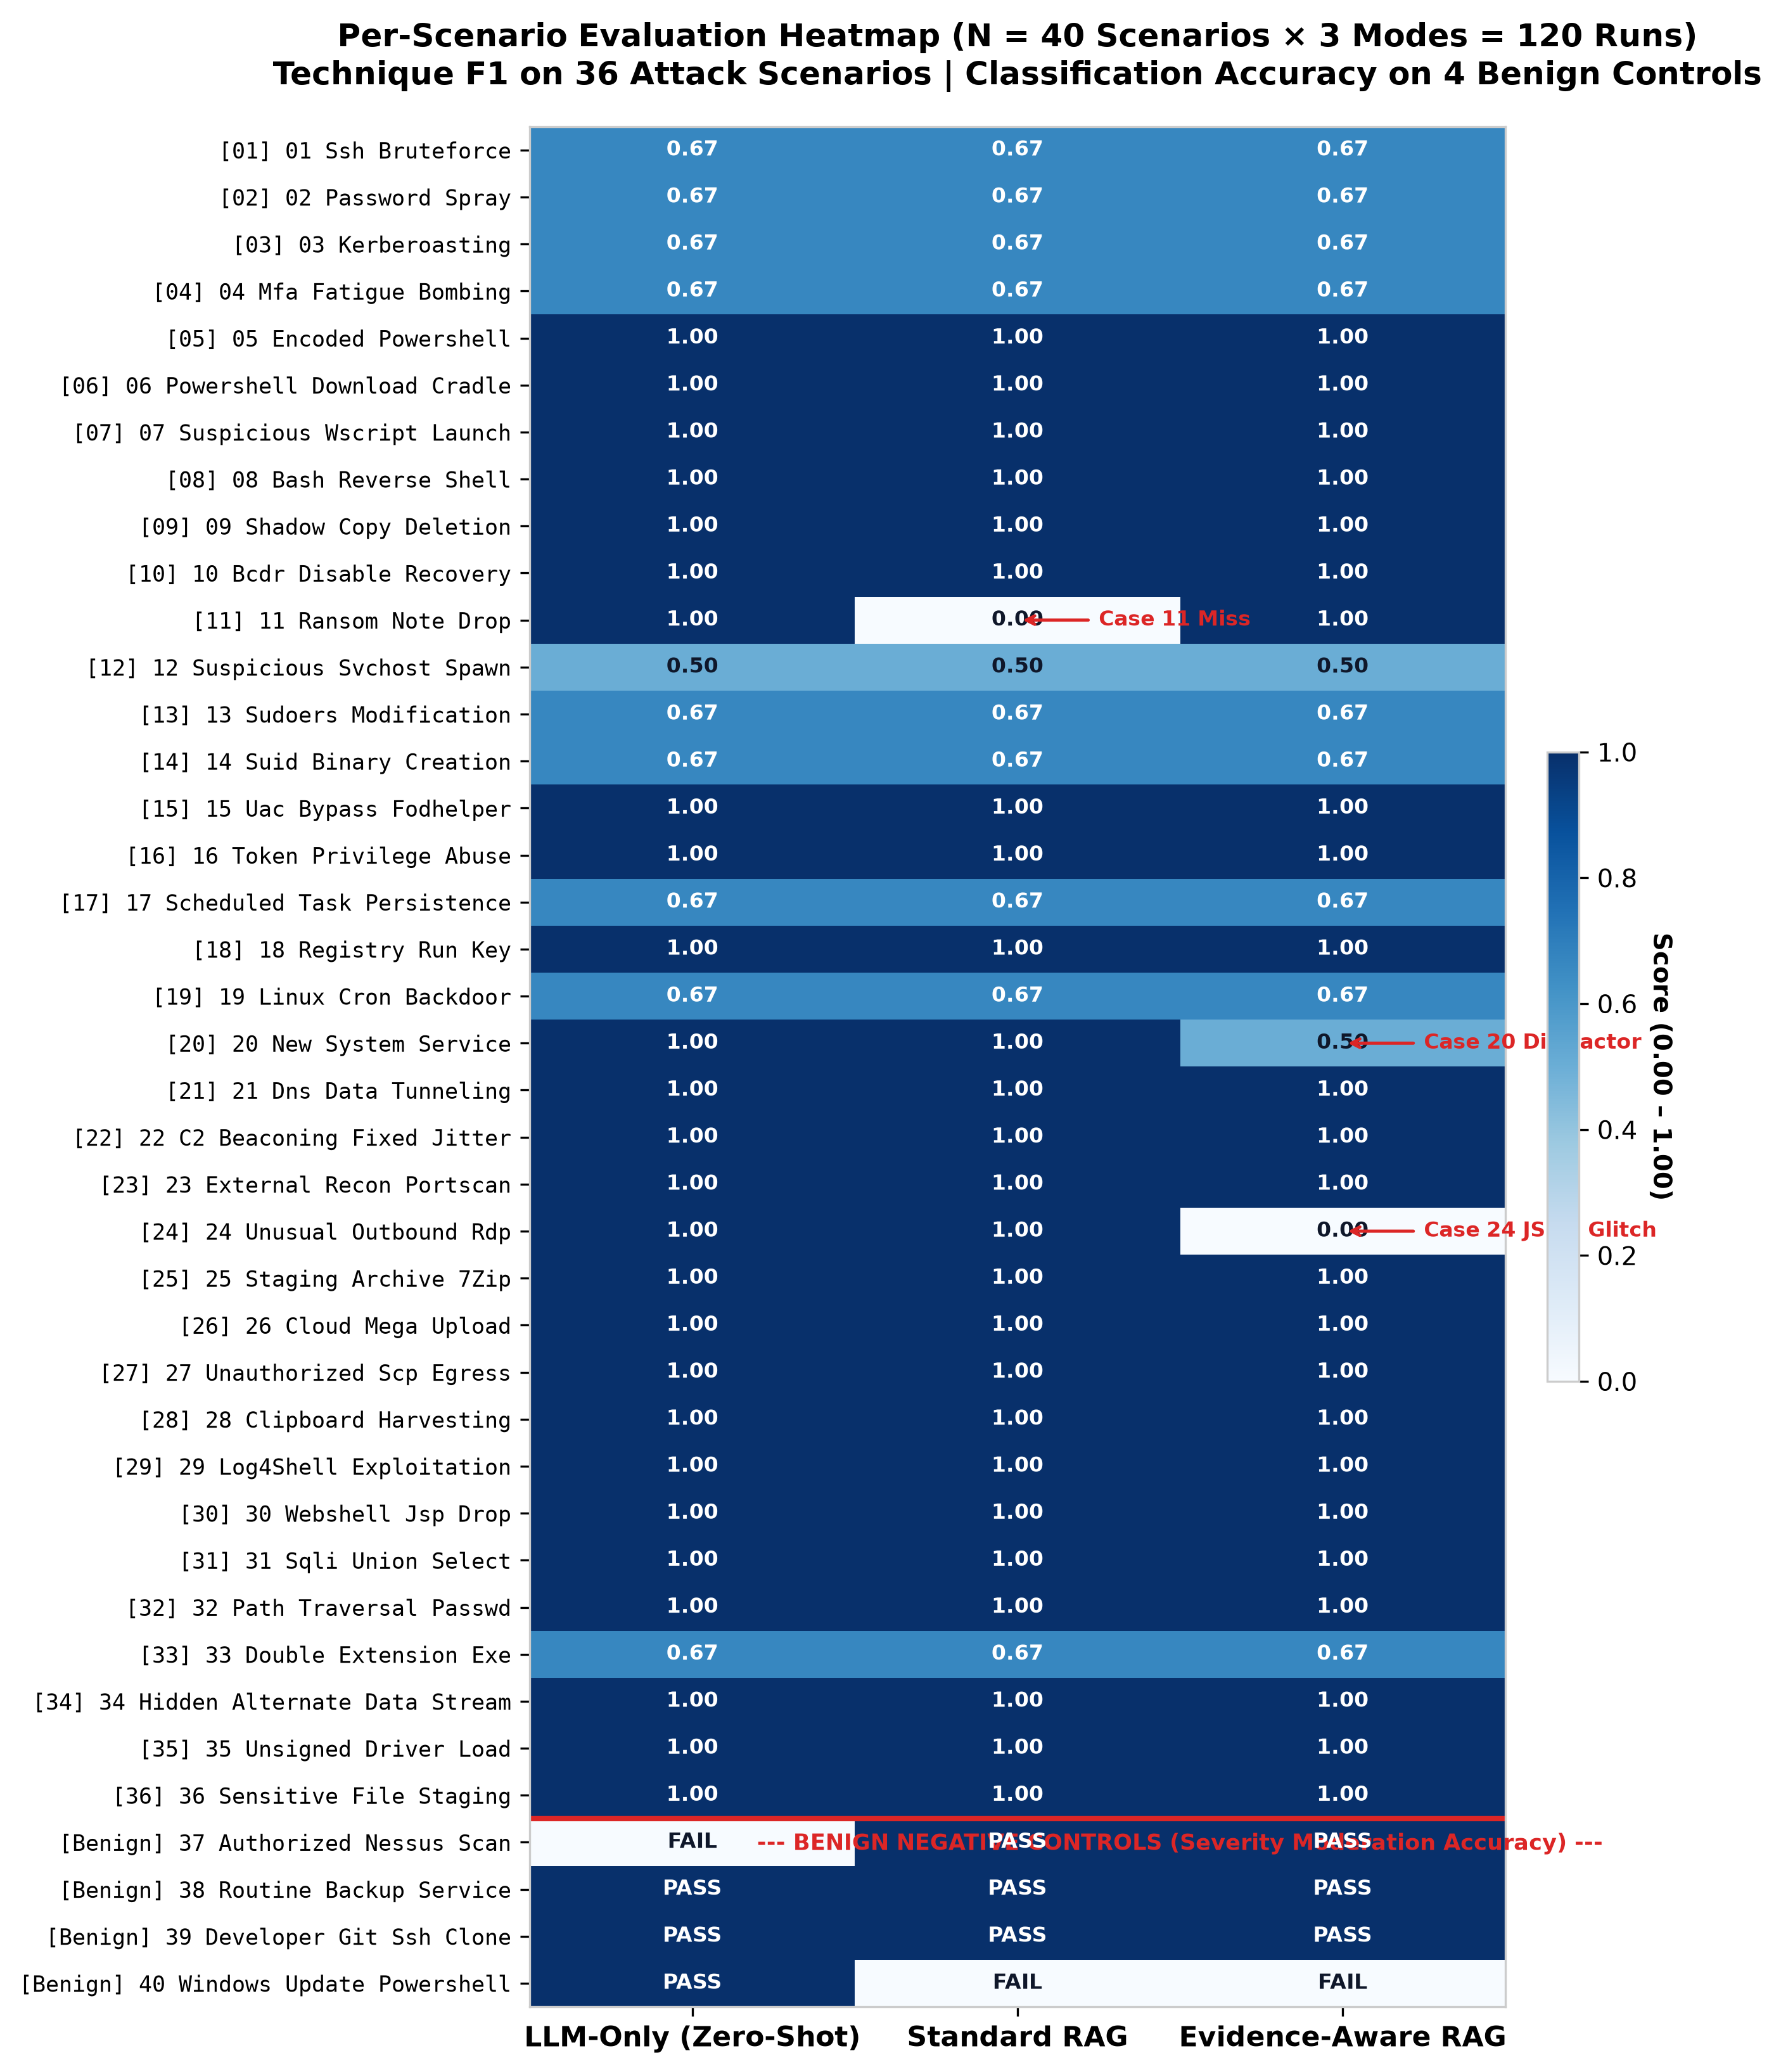
\includegraphics[width=\linewidth,height=5.6cm,keepaspectratio]{figures/figure5_scenario_heatmap.png}
\end{center}

\column{0.54\textwidth}
\SOCcard{\linewidth}{Statistical Structure \& Findings}{
\begin{itemize}\setlength{\itemsep}{1.2pt}\scriptsize
  \item \textbf{Uniform Sample Size}: All 10 categories have an exact, uniform sample size of $N=4$ scenarios ($4 \times 10 = 40$ cases).
  \item \textbf{Consistent Performance}: 1.00 F1 across Credential Access, Execution, Impact, Privilege Escalation, and Persistence.
  \item \textbf{The 3 Specific Attack Outliers}:
    \begin{itemize}\scriptsize
      \item \textit{Case 11 (Ransomware)}: Standard RAG missed (F1: 0.0 vs 1.0).
      \item \textit{Case 20 (Service)}: Evidence-Aware distractor (F1: 0.50 vs 1.0).
      \item \textit{Case 24 (RDP)}: Evidence-Aware JSON glitch (F1: 0.0 vs 1.0).
    \end{itemize}
  \item \textbf{Benign Controls (Rows 37--40)}:
    \begin{itemize}\scriptsize
      \item 75.0\% accuracy (3/4) across all modes.
      \item RAG moderated Nessus scanner (Medium vs High).
    \end{itemize}
\end{itemize}
}
\end{columns}
}

% =============================================================================
% SLIDE 13: CVE Grounding: Log4Shell Case Study
% =============================================================================
\SOCslide{CVE Grounding: Log4Shell Case Study}{Why Parametric LLMs Fail on Specific CVEs While RAG Succeeds}{
\begin{center}
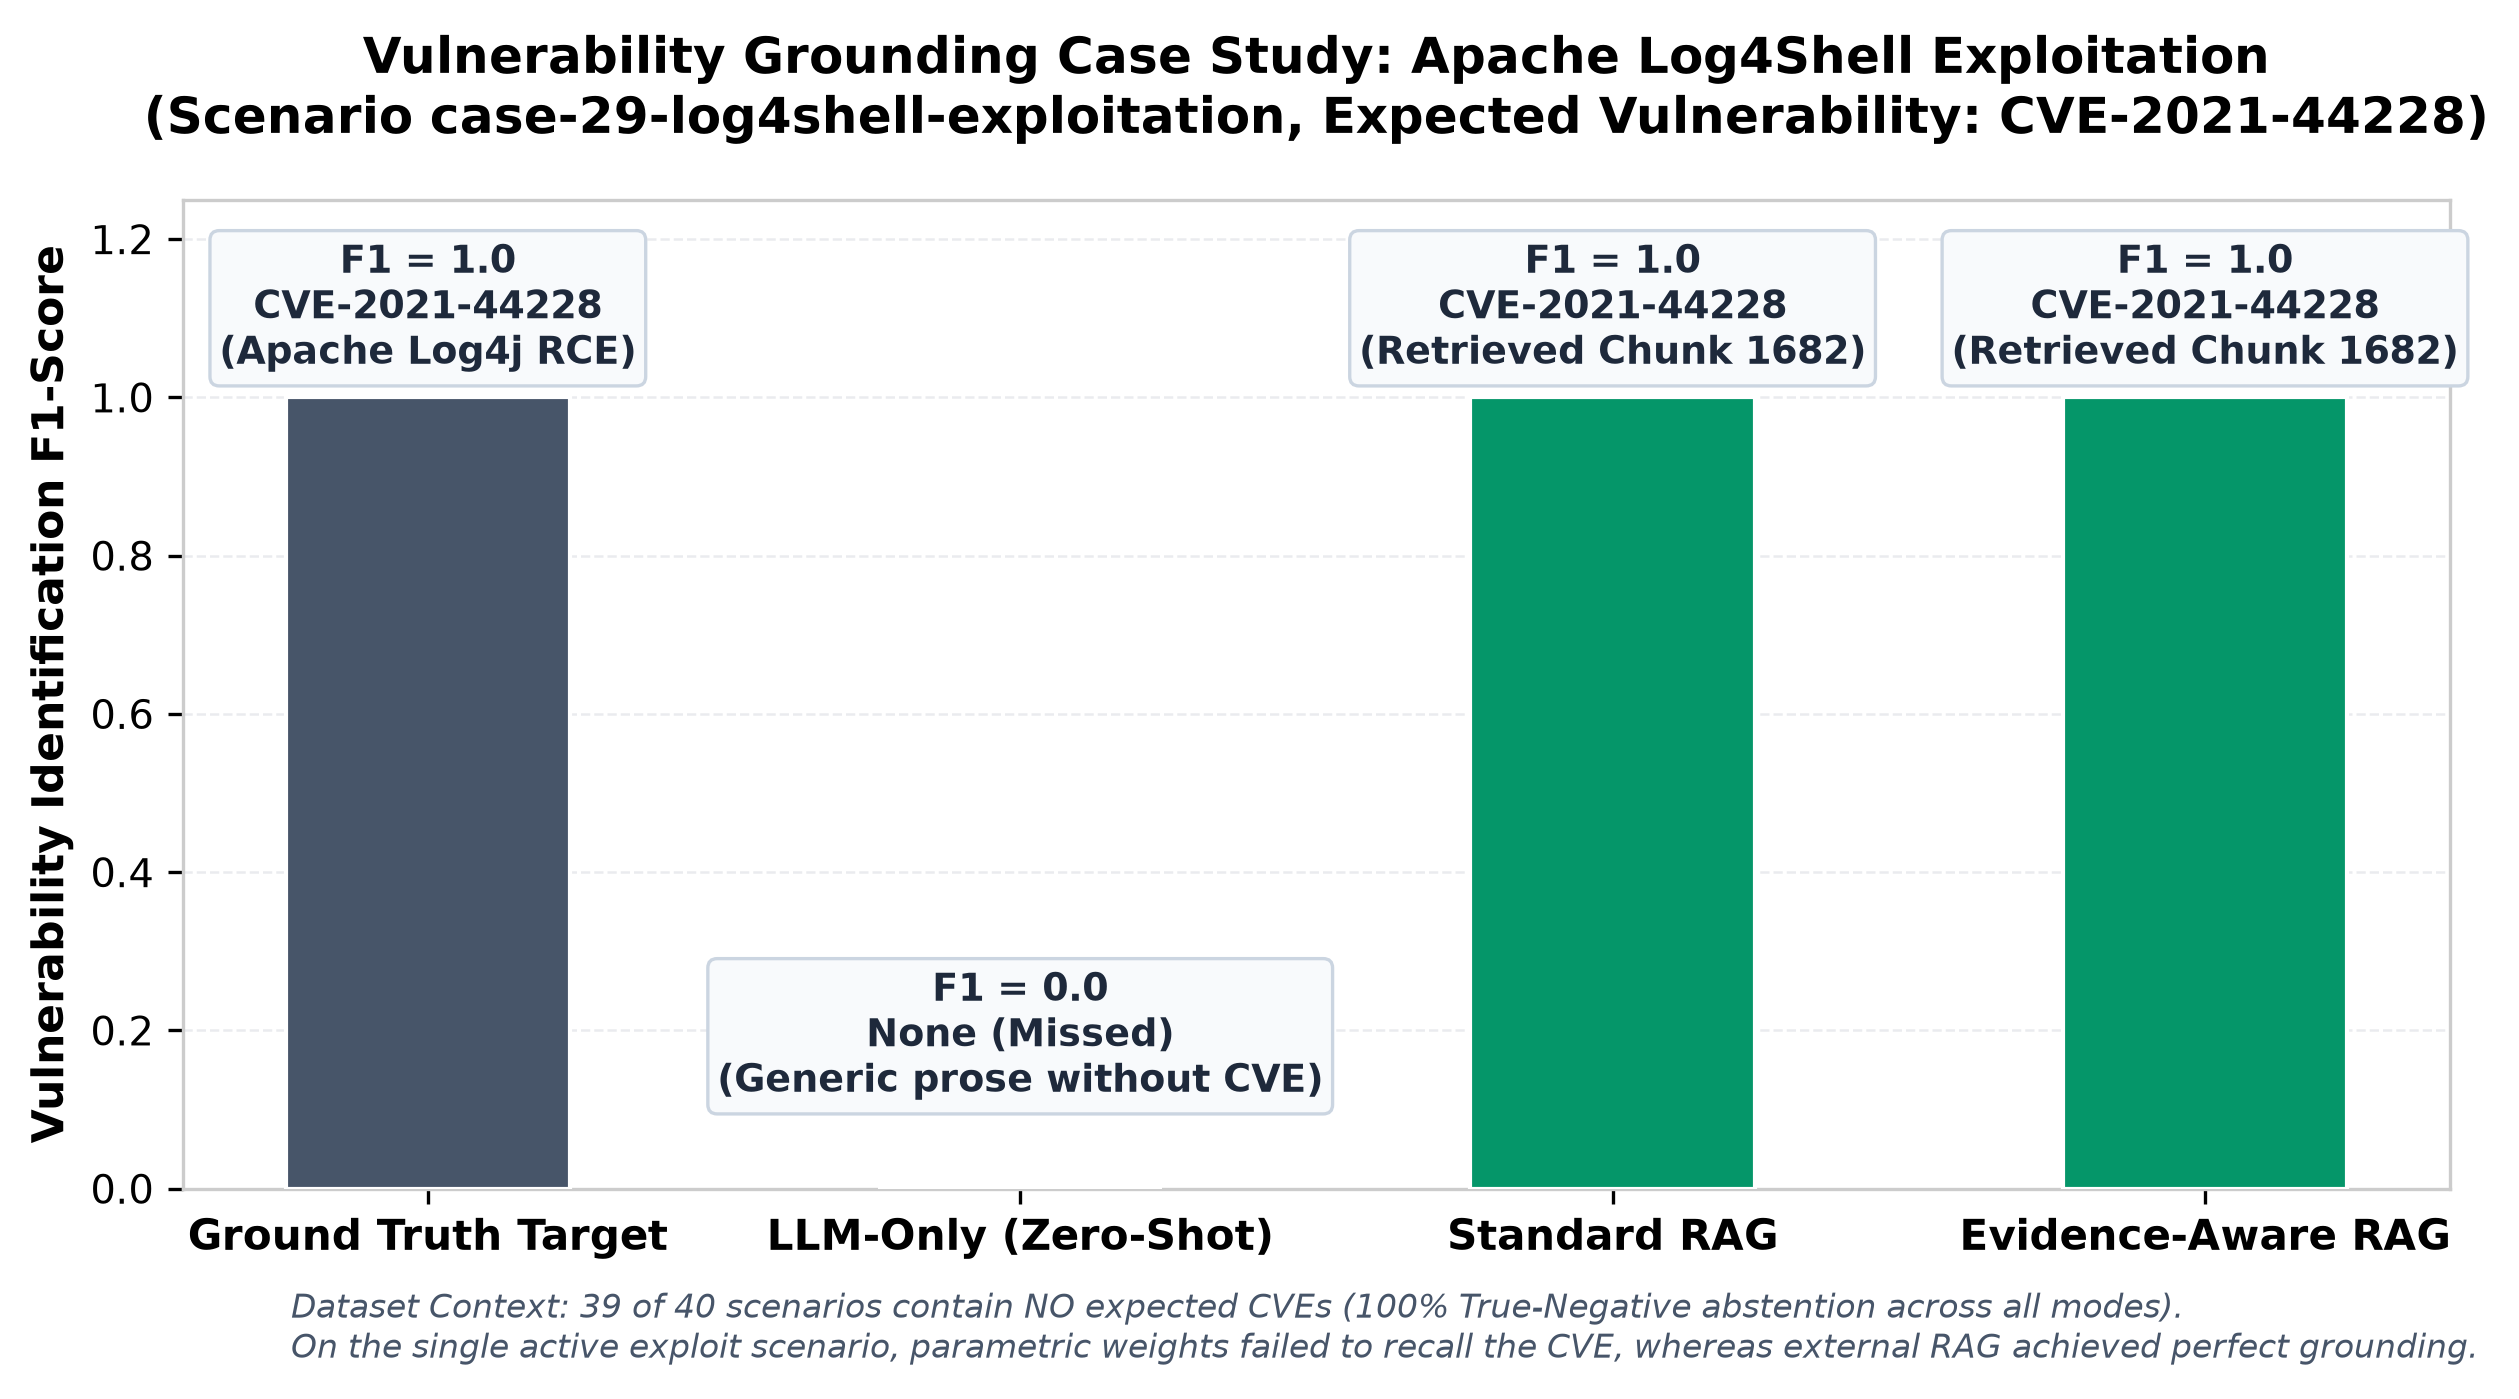
\includegraphics[width=0.96\linewidth,height=4.4cm,keepaspectratio]{figures/figure7_cve_grounding.png}
\end{center}

\vspace{-0.15cm}
\SOCbox{\linewidth}{SOCline}{SOCpale}{
  \footnotesize\textbf{Critical Finding:} While parametric LLMs can recognize broad attack categories from pre-training, \textbf{external RAG is strictly necessary} for authoritative CVE attribution (Log4Shell F1: 1.0 vs 0.0). Across 39 non-CVE scenarios, all modes achieved 100\% True-Negative abstention.
}
}

% =============================================================================
% SLIDE 14: Benign Negative Controls & Citation Veracity
% =============================================================================
\SOCslide{Integrity \& Governance}{Benign False-Alarm Evaluation and Citation Audit Integrity}{
\begin{center}
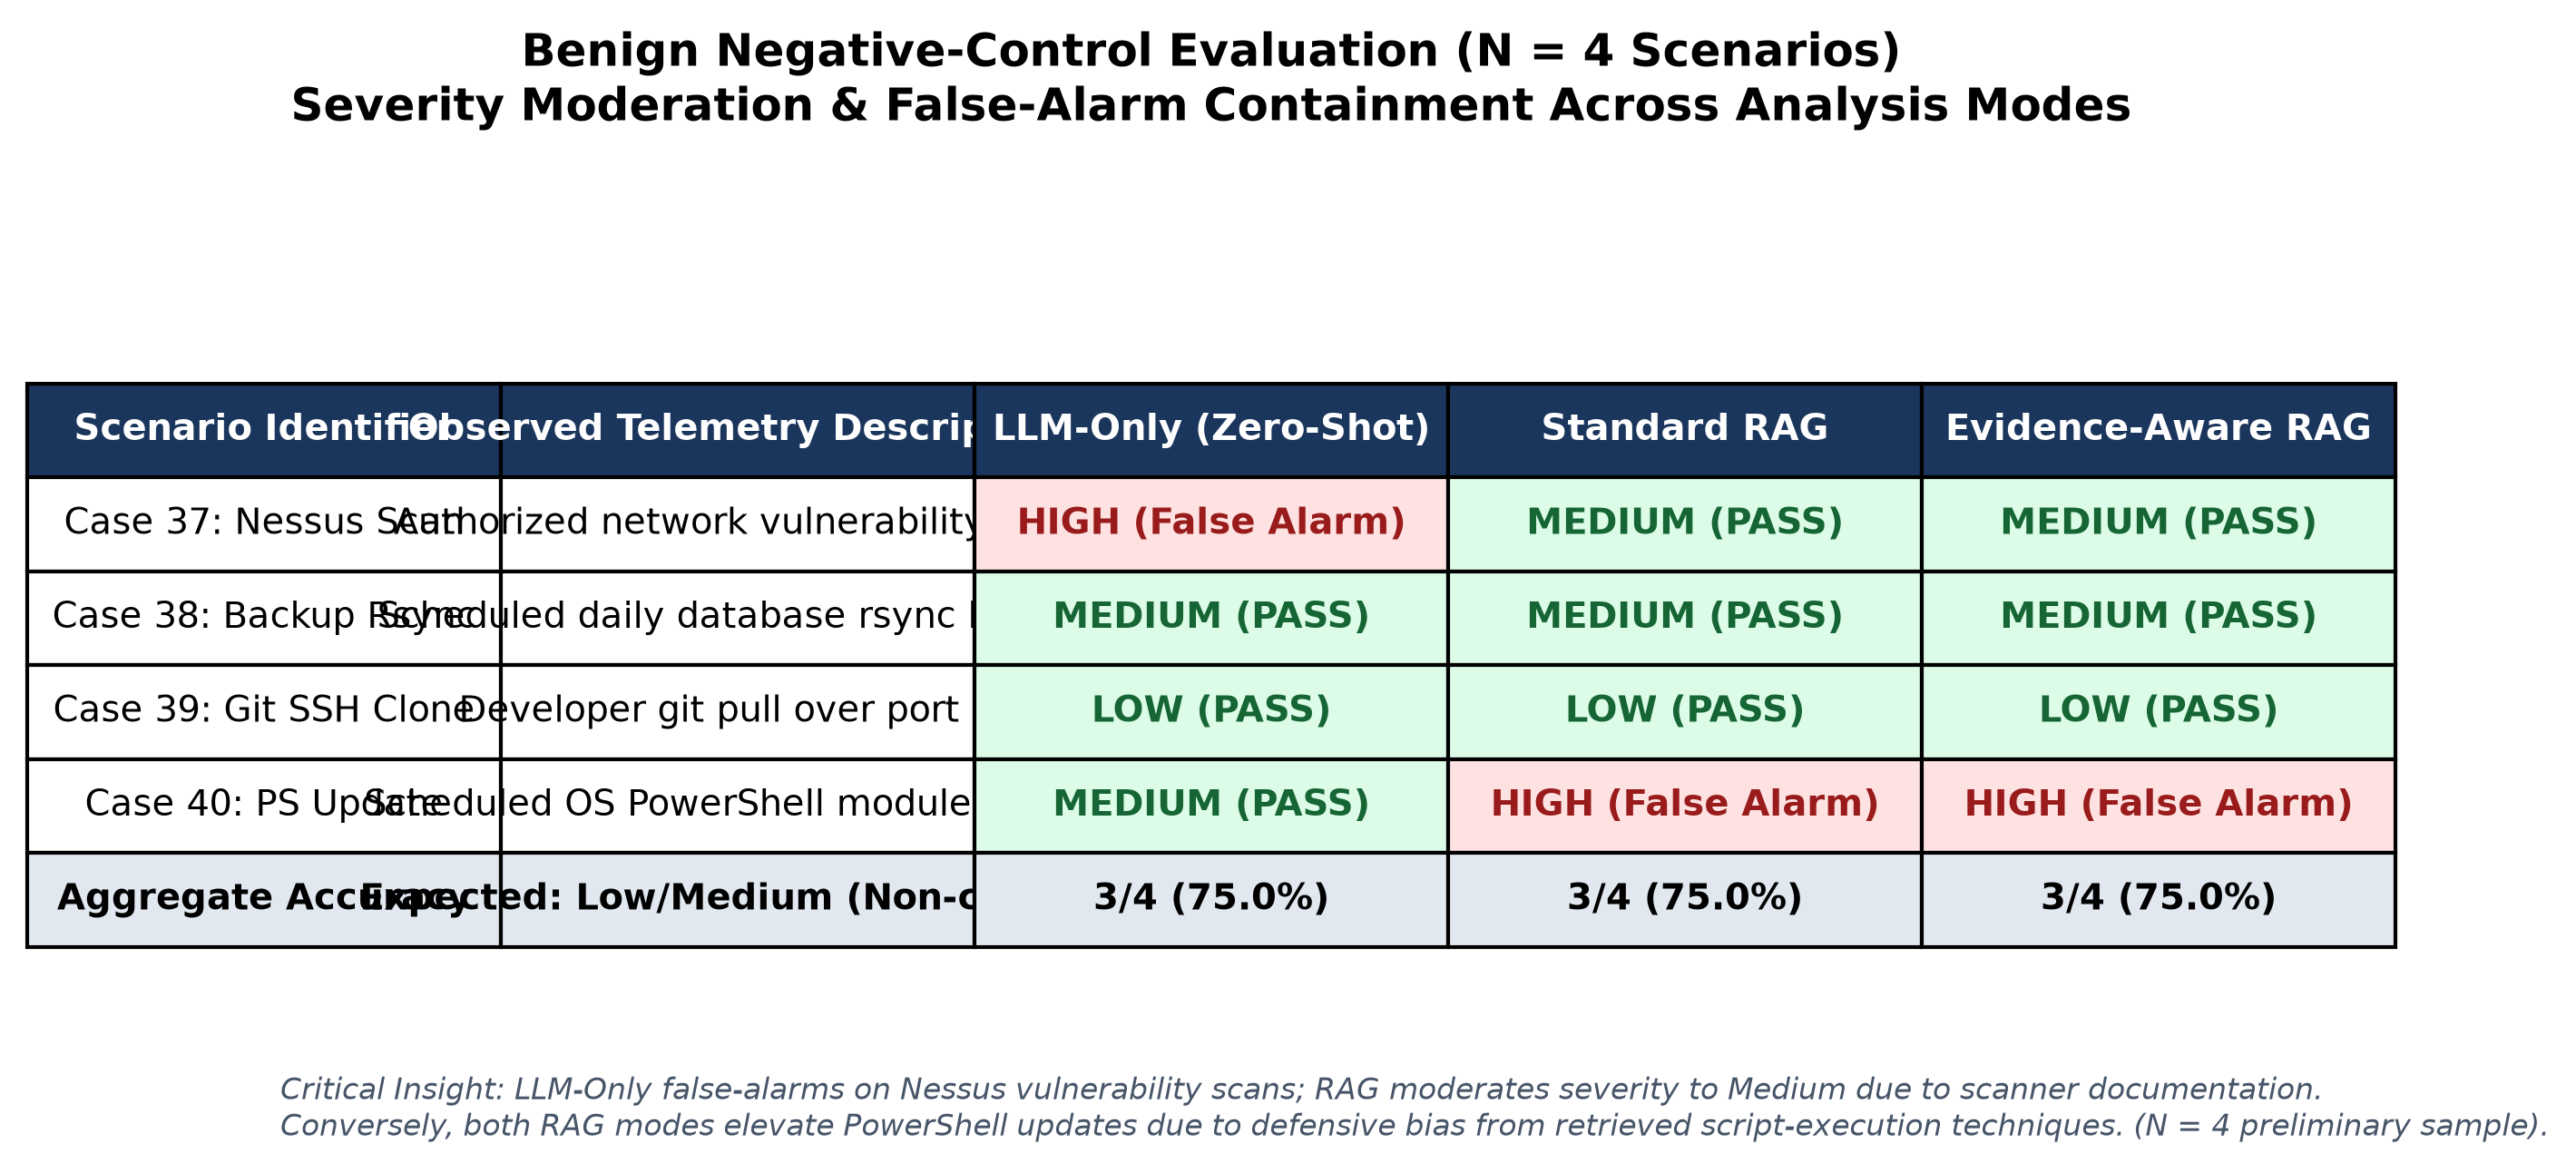
\includegraphics[width=0.96\linewidth,height=3.0cm,keepaspectratio]{figures/figure6_benign_controls.png}
\end{center}

\vspace{-0.22cm}
\begin{columns}[T,onlytextwidth]
\column{0.48\textwidth}
\SOCcard{\linewidth}{Severity Moderation ($N=4$ Preliminary)}{
\begin{itemize}\setlength{\itemsep}{1pt}\scriptsize
  \item \textbf{75.0\% Accuracy}: 3 of 4 cases correctly non-malicious.
  \item \textbf{Nessus Scan (Case 37)}: RAG moderated severity to Medium based on scanner context, preventing false alarm escalation.
  \item \textbf{PowerShell (Case 40)}: Elevated to High by defensive caution.
\end{itemize}
}

\column{0.48\textwidth}
\SOCcard{\linewidth}{Citation Reference Veracity}{
\begin{itemize}\setlength{\itemsep}{1pt}\scriptsize
  \item \textbf{97.3\% Valid Reference Rate}: 36 of 37 cited evidence IDs verified to exist in retrieved threat documentation.
  \item \textbf{Anomaly Detected}: Actively trapped invented ID in Case 22.
  \item \textbf{Scope}: Confirms reference-ID existence and provenance.
\end{itemize}
}
\end{columns}

\vspace{0.04cm}
\SOCbox{\linewidth}{SOCline}{white}{
  \scriptsize\textbf{Governance Value:} Automated citation verification guarantees auditability: human analysts can trace every threat claim back to verifiable MITRE ATT\&CK documentation in the local knowledge base.
}
}

% =============================================================================
% SLIDE 15: Failure Analysis & Limitations
% =============================================================================
\SOCslide{Failure Analysis \& Limitations}{Explaining Why LLM-Only Scored Higher F1 Than Evidence-Aware RAG}{
\SOCbox{\linewidth}{SOCbadgeBg}{SOCpale}{
  \scriptsize\textbf{\color{SOCdark}Key Discovery:} On \textbf{34 of 36 attack scenarios}, LLM-Only and Evidence-Aware RAG achieved \textbf{identical technique F1}. The performance difference stems from exactly \textbf{two edge cases}:
}

\vspace{0.02cm}
\begin{columns}[T,onlytextwidth]
\column{0.48\textwidth}
\SOCcard{\linewidth}{1. Context Distractor Effect (\texttt{case-20})}{
\begin{itemize}\setlength{\itemsep}{1pt}\scriptsize
  \item \textbf{Scenario}: New system service creation (\texttt{T1543.003}).
  \item \textbf{What Happened}: Retrieved ATT\&CK chunk mentioned related technique \texttt{T1036} (Masquerading) and deprecated technique \texttt{T1050}.
  \item \textbf{Consequence}: The 8B LLM over-extrapolated and predicted both as additional techniques, generating \textbf{2 False Positives} (F1 dropped from 1.00 to 0.50).
  \item \textit{Lesson: Rich context can distract small models into over-prediction.}
\end{itemize}
}

\column{0.48\textwidth}
\SOCcard{\linewidth}{2. JSON Syntax Generation Failure (\texttt{case-24})}{
\begin{itemize}\setlength{\itemsep}{1pt}\scriptsize
  \item \textbf{Scenario}: Unusual outbound RDP session (\texttt{T1021.001}).
  \item \textbf{What Happened}: Retrieval correctly pinpointed \texttt{T1021.001}, but \texttt{qwen3:8b} produced malformed markdown instead of pure JSON.
  \item \textbf{Consequence}: JSON parser failed; safe error recovery returned an empty prediction (F1 dropped from 1.00 to \textbf{0.00}).
  \item \textit{Lesson: Structural output formatting requires automated schema repair.}
\end{itemize}
}
\end{columns}

\vspace{0.02cm}
\SOCbox{\linewidth}{SOCline}{SOCpale}{
  \scriptsize\textbf{Operational Scope Limitation:} The benchmark utilizes MITRE tags present in Wazuh rule XML metadata (\texttt{rule.mitre.id}) as operational inputs. Autonomous discovery on raw, un-tagged logs remains an untested boundary.
}
}

% =============================================================================
% SLIDE 16: Testing & Validation
% =============================================================================
\SOCslide{Testing \& Validation}{Multi-Tier Automated Test Suite and Benchmark Regression Verification}{
\begin{columns}[T,onlytextwidth]
\column{0.48\textwidth}
\SOCcard{\linewidth}{258 Automated Software Tests}{
\begin{itemize}\setlength{\itemsep}{2pt}\footnotesize
  \item \textbf{Backend Pytest Suite (\textcolor{SOCgreen}{226 passed}, 0 failed)}:
    \begin{itemize}\scriptsize
      \item Telemetry normalization, entity extraction, deduplication.
      \item Qdrant vector retrieval, hybrid filters, payload validation.
      \item Tri-mode orchestration and citation integrity verification.
      \item Wazuh transport client and API error recovery.
    \end{itemize}
  \item \textbf{Frontend Vitest Suite (\textcolor{SOCgreen}{32 passed}, 0 failed)}:
    \begin{itemize}\scriptsize
      \item Triage console, live trace viewer, interactive entity graph.
      \item Clean production build verified in 4.9 seconds.
    \end{itemize}
\end{itemize}
}

\column{0.48\textwidth}
\SOCcard{\linewidth}{Dedicated Benchmark Integrity Suite}{
\begin{itemize}\setlength{\itemsep}{2.5pt}\footnotesize
  \item \textbf{6 Automated Integrity Tests (\textcolor{SOCgreen}{6 passed})}:
    \begin{itemize}\scriptsize
      \item \textbf{Zero Collision Guarantee}: Verifies \texttt{v2-eval-xxx} alert IDs never collide with historical v1 data.
      \item \textbf{Schema Integrity}: Confirms database column \texttt{alerts.data\_source} is migrated and correctly populated.
      \item \textbf{Idempotent Seeding}: Proves benchmarks can be resumed cleanly without duplicating alert records.
    \end{itemize}
  \item \textbf{Non-Destructive Testing Fixture}: Uses transactional savepoints and engine disposal to prevent connection leaks.
\end{itemize}
}
\end{columns}

\vspace{0.08cm}
\SOCbox{\linewidth}{SOCline}{SOCpale}{
  \footnotesize\textbf{Testing Distinction:} Software tests (258 passed) verify system correctness, API stability, and data integrity; detection capabilities are evaluated separately on the 120 benchmark runs.
}
}

% =============================================================================
% SLIDE 17: Technical Contributions & Innovation
% =============================================================================
\SOCslide{Technical Contributions \& Innovation}{Four Concrete Engineering and Research Contributions for PPD-II}{
\begin{columns}[T,onlytextwidth]
\column{0.48\textwidth}
\SOCcard{\linewidth}{1. Entity-Anchored Retrieval (+67.5\% Recall@1)}{
\begin{itemize}\setlength{\itemsep}{2pt}\scriptsize
  \item Identified and formulated the \textbf{semantic drift failure mode} of standard dense RAG on unstructured security telemetry.
  \item Engineered an entity-anchored hybrid retrieval pipeline that boosts Recall@1 from \textbf{22.5\% to 90.0\%} ($MRR: 0.2742 \to 0.9125$).
\end{itemize}
}

\vspace{0.08cm}
\SOCcard{\linewidth}{2. Sovereign On-Premise SOC Architecture}{
\begin{itemize}\setlength{\itemsep}{2pt}\scriptsize
  \item Implemented a fully local, zero-cloud triage architecture combining FastAPI, PostgreSQL, Qdrant, and Ollama (\texttt{qwen3:8b}).
  \item Eliminates enterprise data leakage and external API billing.
\end{itemize}
}

\column{0.48\textwidth}
\SOCcard{\linewidth}{3. Verifiable Citation Integrity Governance}{
\begin{itemize}\setlength{\itemsep}{2pt}\scriptsize
  \item Implemented automated reference verification that cross-checks LLM citations against retrieved evidence IDs (\textbf{97.3\% valid}).
  \item Actively detects and penalizes invented citation references.
\end{itemize}
}

\vspace{0.08cm}
\SOCcard{\linewidth}{4. Reproducible Tri-Mode Benchmark \& Audit}{
\begin{itemize}\setlength{\itemsep}{2pt}\scriptsize
  \item Completed 120 controlled evaluations across 40 curated scenarios.
  \item Produced an independently audited research report with full trajectory preservation and rigorous failure analysis.
\end{itemize}
}
\end{columns}
}

% =============================================================================
% SLIDE 18: Implementation Status & Future Work
% =============================================================================
\SOCslide{Implementation Status \& Roadmap}{Milestones Achieved for Review 3 and Clear Roadmap to Final Defense}{
\begin{columns}[T,onlytextwidth]
\column{0.48\textwidth}
\SOCcard{\linewidth}{Third Review Milestones (100\% Complete)}{
\begin{itemize}\setlength{\itemsep}{2pt}\footnotesize
  \item \textcolor{SOCgreen}{\textbf{$\checkmark$ Database Migration}}: Schema upgraded to \texttt{c01\_datasource} with strict data-source separation.
  \item \textcolor{SOCgreen}{\textbf{$\checkmark$ Benchmark Completion}}: All 120 evaluations across 40 Dataset v2 scenarios executed without errors.
  \item \textcolor{SOCgreen}{\textbf{$\checkmark$ Integrity Audit}}: Zero-collision verification and retrieval ablation completed ($N=40$).
  \item \textcolor{SOCgreen}{\textbf{$\checkmark$ Publication Assets}}: 5 high-resolution figures and 4 LaTeX tables prepared.
\end{itemize}
}

\column{0.48\textwidth}
\SOCcard{\linewidth}{Roadmap to Final Defense (Fourth Review)}{
\begin{itemize}\setlength{\itemsep}{2pt}\footnotesize
  \item \textbf{1. Historical Trace Persistence}: Store real per-stage execution durations in PostgreSQL rather than synthetic estimates.
  \item \textbf{2. Live Wazuh SIEM Deployment}: Connect verified OpenSearch transport client to a dedicated remote Wazuh cluster.
  \item \textbf{3. Distractor Suppression}: Add prompt constraints to prevent contextual over-prediction (resolving Case 20).
  \item \textbf{4. Automated Schema Repair}: Implement JSON fallback repair to eliminate formatting failures (resolving Case 24).
\end{itemize}
}
\end{columns}

\vspace{0.08cm}
\SOCbox{\linewidth}{SOCline}{SOCpale}{
  \footnotesize\textbf{Current State:} The assistant is a fully operational, locally deployed research prototype with verified empirical findings, ready for live demonstration.
}
}

% =============================================================================
% SLIDE 19: Conclusion & Questions
% =============================================================================
\SOCslide{Conclusion}{Summary of PPD-II Third Review Achievements}{
\begin{columns}[T,onlytextwidth]
\column{0.53\textwidth}
\SOCcard{\linewidth}{Summary of Deliverables}{
\begin{itemize}\setlength{\itemsep}{2.5pt}\footnotesize
  \item \textbf{Operational System}: Sovereign, audit-ready SOC assistant integrating FastAPI, PostgreSQL, Qdrant, Ollama, and React 19.
  \item \textbf{Retrieval Breakthrough}: Entity anchoring achieves a \textbf{+67.5 percentage-point leap in Recall@1} over standard dense RAG (90.0\% vs 22.5\%).
  \item \textbf{Critical Scientific Nuance}: Zero-shot LLM leads on broad classification F1 (0.9028 vs 0.8611), but RAG is indispensable for precise CVE grounding (Log4Shell F1: 1.0 vs 0.0) and citation auditability (97.3\% validity).
  \item \textbf{Verified Code Quality}: 258 automated tests passing; 120 benchmark evaluations audited with zero collisions.
\end{itemize}
}

\column{0.44\textwidth}
\begin{tcolorbox}[
  colback=SOCteal,colframe=SOCteal,arc=2mm,center,top=6pt,bottom=6pt,
  drop shadow={opacity=.12,shadow xshift=1pt,shadow yshift=-1pt}
]
  \centering
  \textcolor{white}{\large\bfseries Thank You!}\\[4pt]
  \textcolor{SOCtealLight!40}{\small\textbf{Questions \& Discussion}}\\[8pt]
  \textcolor{white!95}{\footnotesize\textbf{Project Team}}\\[2pt]
  \textcolor{white!85}{\scriptsize Kunal Sanga (2301341031)}\\[1pt]
  \textcolor{white!85}{\scriptsize Soumili Ghosh (231341057)}\\[1pt]
  \textcolor{white!85}{\scriptsize Bivan Jena (2301341021)}\\[5pt]
  \textcolor{white!90}{\scriptsize\textbf{Guide:} Miss Alka Dash}\\[1pt]
  \textcolor{white!70}{\tiny Assistant Professor, Department of CSE}\\[2pt]
  \textcolor{white!60}{\tiny Silicon Institute of Technology, Sambalpur}
\end{tcolorbox}
\end{columns}
}

\end{document}
